
% \part{复变函数论}

% \chapter{复变函数论}
% \label{chap:complexfunctions}

\chapter{复数和复变函数}
\begin{introduction}
\item 复数
\item 复变函数
\item 复变函数积分
\item 复数级数
\item 留数定理及应用
\item 费曼技巧
\end{introduction}

复变函数论是物理学和工程学广泛使用的强大分析工具,学习掌握这个理论十分必要.
\section{复数}
% \part{复变函数论}

\chapter{复变函数论}
\label{chap:complexfunctions}
复变函数论是物理学和工程学广泛使用的强大分析工具,学习掌握这个理论十分必要。
\section{复数和复变函数}
\subsection{复数的定义和基本性质}
\subsubsection{定义}
一元二次方程$a x^2 + b x + c = 0 (a\neq 0, b,c \in \mathbb{R})$的求解大家一定都不陌生。当$\Delta \equiv b^2 - 4 a c \geq 0$时,方程有解,求根公式可得
\begin{equation}
    x = \frac{-b \pm \sqrt{\Delta}}{2a} \textrm{。}
\end{equation}
当$\Delta < 0$时,方程无解。这里的无解其实是指没有实数解。
当我们引入以下这一核心定义后,
\begin{equation}
    \imath ^2 = -1 \quad \textrm{或} \quad \imath = \sqrt{-1} \textrm{。} 
\end{equation}
$\imath$为{\bf 虚数},将定义域扩展到复数,二次方程就有确定的两个解,当$\Delta < 0$时,方程有两个复数解:
\begin{equation}
    x = \frac{-b \pm \imath \sqrt{-\Delta}}{2a} \textrm{。}
\end{equation}
复数$z$定义为
\begin{equation}
    \label{eq:complex_alg}
    z = x + \imath \; y \textrm{,}
\end{equation}
$x,y \in {\mathbb{R}}$。$x,y$分别为复数$z$的{\bf 实部}(real part) 和{\bf 虚部}(imaginary part)。
上式\eqref{eq:complex_alg}成为复数的代数式。复数域常用$\mathbb{C}$来表示。若将$z$看成是由$x,y$组成的有序对$(x,y)$,记为
\begin{equation}
    z \equiv (x,y)\textrm{,}
\end{equation}
则有$1 = (1,0), \imath = (0, 1)$。如果将$x,y$当做平面上点的坐标,复数$z$就和平面上的点一一对应起来。
形成的平面叫做{\bf 复数平面},坐标轴成为{\bf 实轴}和{\bf 虚轴}。
\begin{figure}[htb]
    \centering
    \begin{tikzpicture}[scale=1.5]
    \path (0,0) coordinate (origin);
    \path (4, 0) coordinate (x) ;
    \path (0, 2.5) coordinate (y) ;
    \path (4, 2.5) coordinate (z);
    \path (2.5, 2) coordinate (rho);
  
    \draw[->] (-0.2,0) --(4.2,0) node[right] {$\Re$};
    \draw[->] (0,-0.2) --(0,3.2) node[above] {$\Im$};
    \draw[solid, text=blue, thick, -{Stealth[length=2mm]}] (origin) -- (z) node[above] {$z=\rho e^{\imath \varphi}$};
    \draw[text=red, dashed]  (x) --(z) node[above]  {};
    \draw[text=red, dashed] (y) --(z) node[above] {};
  
    \node at (origin) [below] {$O$};
    \node at (x) [below ]{$x$};
    \node at (y) [left ]{ $y$};
    \node at (rho) [right] {$\rho$};
    \draw[color=red, fill=red] (z) circle (0.05);
  
    \draw pic["$\varphi$",draw, ->, angle eccentricity=1.2, angle radius=0.8cm]{angle = x--origin--z};
  
  \end{tikzpicture}
  \caption{复数的平面表示。} \label{fig:complex_plane}
\end{figure} 
自然我们可以改用极坐标来表示,
\begin{align}
    & \rho = \sqrt{x^2 + y^2}\\
    & \varphi = \arctan y/x
\end{align}
或
\begin{align}
    & x = \rho \cos\varphi \\
    & y = \rho \sin\varphi 
\end{align}
则我们得到复数$z$的三角式
\begin{equation}
    z = \rho (\cos\varphi +  \imath\; \sin\varphi) \textrm{,}
\end{equation}
或指数式
\begin{equation}
    z = \rho e^{\imath \varphi} \textrm{。}
\end{equation}
$\rho = |z|$ 为复数的{\bf 模}(modulus), $\varphi$为复数的{\bf 辐角}(argument),记作$\Arg z$。
对于任意一个$z=\rho e^{\imath \varphi}$,由于恒等式$e^{\imath 2\pi n} = 1$, $n = 0, \pm 1, \pm 2, \dots, \in \mathbb{Z}$,
可以知道辐角$\Arg z$不能唯一确定,它们之间相差$2\pi$的整数倍,其中满足
\begin{align}
    0 \leq \Arg z < 2\pi \textrm{,}
\end{align}
的辐角为$z$的主辐角,记为$\arg z$。$\arg z$ 为$\Arg z$的主值。
\begin{align}
    \Arg z = \arg z + 2 n \pi \quad (n = 0, \pm 1, \pm 2\dots)\textrm{。}
\end{align}
\begin{examplebox}{求$\sqrt[3]{-\imath}$。}
    首先,我们有恒等式$e^{\imath 2\pi n} = 1$,且
    \begin{align*}
        e^{\imath \frac{\pi}{2}}  = i & \quad  e^{\imath \pi}  =-1 \\
        e^{\imath \frac{3\pi}{2}} = -i & \quad e^{\imath 2\pi} = 1\textrm{。}
    \end{align*}
题目就是要求方程$z^3 =\sqrt[3]{-\imath}$的根。可以得到
    \begin{align*}
        e^{\frac{1}{3}(\imath 2\pi n + \imath \frac{3\pi}{2})} & = (-i)^{\frac{1}{3}} \\
        e^{(\imath \frac{2}{3}\pi n + \imath \frac{\pi}{2})}   & =  (-i)^{\frac{1}{3}} \\
    \end{align*}
得到的解分三种情况
    \begin{align*}
        z_1 &=e^{\imath \frac{\pi}{2}} = \imath , n = 3k \\
        z_2 &=e^{\imath \frac{7\pi}{6}} = -\frac{\sqrt{3}}{2} - \frac{\imath}{2} , n = 3k +1 \\
        z_3 &=e^{\imath \frac{11\pi}{6}} = -\frac{\sqrt{3}}{2} + \frac{\imath}{2} , n = 3k +1 
    \end{align*}
它们在复平面上的分布如下图所示,它们之间的夹角为$120^\circ$,模为单位长度$1$。
    % \begin{figure}
        \centering 
        \begin{tikzpicture}[scale=1.0]
    \def\sin60{}
    \path (0,0) coordinate (origin);
    \path (0, 1) coordinate (z1) ;
    \path ({-sqrt(3)/2}, -0.5 ) coordinate (z2) ;
    \path ({sqrt(3)/2},  -0.5) coordinate (z3);
  
    \draw[->] (-2,0) --(2,0) node[right] {$\Re$};
    \draw[->] (0,-2) --(0,2) node[above] {$\Im$};
    \draw[solid, text=blue, thick, -{Stealth[length=2mm]}] (origin) -- (z1) node[above] {$z_1$};
    \draw[solid, text=blue, thick, -{Stealth[length=2mm]}] (origin) -- (z2) node[below] {$z_2$};
    \draw[solid, text=blue, thick, -{Stealth[length=2mm]}] (origin) -- (z3) node[below] {$z_3$};
    % \draw[text=red, dashed] (y) --(z) node[above] {};
  
    % \node at (origin) [left] {$O$};
    % \node at (rho) [right] {$\rho$};
    \draw[color=red, dashed] (origin) circle (1);
    % \draw
    \draw[color=red, fill=red] (z1) circle (0.05);
    \draw[color=red, fill=red] (z2) circle (0.05);
    \draw[color=red, fill=red] (z3) circle (0.05);
    % \draw pic["$\varphi$",draw, ->, angle eccentricity=1.2, angle radius=0.8cm]{angle = x--origin--z};
    % \draw pic["$\varphi$",draw, <-, angle eccentricity=1.2, angle radius=0.8cm]{angle = zminus--origin--x};

  \end{tikzpicture}
    % \end{figure}
\end{examplebox}

\subsubsection{基本性质}
我们可以利用有序实数对的方式对复数进行基本运算: 加减乘除运算。{\bf 加法}运算可以定义为
\begin{align}
    z_1 + z_2 = (x_1, y_1) + (x_2, y_2) = (x_1 + x_2, y_1 + y_2) \textrm{。}
\end{align}
{\bf 乘法}运算定义为
\begin{align}
    z_1 \cdot z_2 = (x_1, y_1) \cdot (x_2, y_2) = (x_1 x_2 - y_1 y_2, x_1 y_2 + x_2 y_1) \textrm{。}
\end{align}
显然加法和乘法满足{\bf 交换律}和{\bf 结合律},以后乘法运算符号$\cdot$均省略。
同实数一样,根据以上定义我们可以得到复数域中的一些特殊元素。对于任意复数$z$,复数域中存在元素$e$满足以下性质
\begin{align}
    & e + z = z + e = z \textrm{,}\\ 
    & e \cdot z = z \cdot e = z \textrm{,} 
\end{align}
可以得到对应的分别为
\begin{align}
    (0, 0) &= 0\\
    (1, 0) &= 1 \textrm{,}
\end{align}
通过元素$(0,0)$,我们可以定义$-z$使得 $-z + z = 0$。 于是有,$- z = (-x, -y)$。于是我们定义
{\bf 减法}运算为 
\begin{align}
    z_1 - z_2 \equiv z_1 + (-z_2) = (x_1 - x_2, y_1 - y_2) \textrm{,}
\end{align}
通过元素$(1,0)$,我们定义$z^{-1}$使得
$z^{-1} \cdot z = 1$,于是有 $z^{-1} =e^{-\imath \varphi}/\rho  $。
或$z^{-1} = (\frac{x}{x^2 + y^2}, -\frac{y}{x^2 + y^2})$。{\bf 除法}运算定义为
\begin{align}
    z_1 / z_2 \equiv z_1 \cdot z_2^{-1} = \frac{x_1 x_2 - y_1 y_2} {x_2^2  +  y_2^2 }  + \imath \frac{y_1 x_2 - x_1 y_2} {x_2^2  +  y_2^2 } \textrm{。} 
\end{align}
注意往往乘除写成极坐标表达更简洁:
\begin{align}
    z_1 z_2 = \rho_1 e^{\imath \varphi_1 } \rho_2 e^{\imath \varphi_2 } = \rho_1 \rho_2 e^{\imath (\varphi_1 + \varphi_2)}
\end{align}

此外,复数还有一种运算较为特殊,称为{\bf 共轭}(complex conjugation)运算。共轭运算表示为
\begin{align}
    z^{*} \equiv (x, -y) = x - \imath y \textrm{。}
\end{align}
为了得到$z$的模,我们可以利用共轭运算,$|z| = \sqrt{zz^{*}}$。注意区分$|z|^2$和$z^2$的不同。

部分复数运算可以映射到复平面上。如共轭运算可以理解为对$z$以实轴为对称轴的镜面对称。对任意的$z_1,z_2$,它们的加减
同向量的加减完全等价,由三角形的三边关系可得
\begin{equation}
    \left| |z|- |z'| \right| \leq |z \pm z'| \leq |z| + |z'| \textrm{。}
\end{equation}
很显然,$z+z^{*} = 2 \Re z$, $z-z^{*} = 2\imath \Im z$。
\begin{figure}
% \begin{minipage}{0.5\textwidth}
% \begin{figure}[htb]
    \centering
    \begin{tikzpicture}[scale=0.8]
    \path (0,0) coordinate (origin);
    \path (4, 0) coordinate (x) ;
    \path (0, 2.5) coordinate (y) ;
    \path (3, 2.0) coordinate (z);
    \path (3,-2.0) coordinate (zminus);
    % \path (2.5, 2) coordinate (rho);
  
    \draw[->] (-0.2,0) --(4.2,0) node[right] {$\Re$};
    \draw[->] (0,-2.5) --(0,2.5) node[above] {$\Im$};
    \draw[solid, text=blue, thick, -{Stealth[length=2mm]}] (origin) -- (z) node[above] {$z=\rho e^{\imath \varphi}$};
    \draw[solid, text=blue, thick, -{Stealth[length=2mm]}] (origin) -- (zminus) node[below] {$z^{*}=\rho e^{-\imath \varphi}$};
    \draw[text=red, dashed]  (zminus) --(z) node[above]  {};
    % \draw[text=red, dashed] (y) --(z) node[above] {};
  
    \node at (origin) [left] {$O$};
    \node at (x) [below ]{$x$};
    \node at (y) [left ]{ $y$};
    % \node at (rho) [right] {$\rho$};
    \draw[color=red, fill=red] (z) circle (0.05);
    \draw[color=red, fill=red] (zminus) circle (0.05);
    % \draw pic["$\varphi$",draw, ->, angle eccentricity=1.2, angle radius=0.8cm]{angle = x--origin--z};
    % \draw pic["$\varphi$",draw, <-, angle eccentricity=1.2, angle radius=0.8cm]{angle = zminus--origin--x};

  \end{tikzpicture}
%   \caption{共轭的几何表示。} \label{fig:zminus}
% \end{figure} 
% \end{minipage}
\quad 
% \begin{minipage}{0.5\textwidth}
    % \begin{figure}[htb]
        % \centering
        \begin{tikzpicture}[scale=0.8]
    % Define the vectors
    \path (3, 2.0) coordinate (z1);
    \path (1, -1.0) coordinate (z2);
    \path (4, 1) coordinate (z1pz2);
    \path (2, 3) coordinate (z1mz2);

    \draw[-{Stealth[length=2mm]}] (0,0) -- (z1) node[midway, above]{$z_1$};
    \draw[-{Stealth[length=2mm]}] (0,0) -- (z2) node[left]{$z_2$};
    % Draw the vector addition
    \draw[-{Stealth[length=2mm]}, text=blue, thick] (0,0) -- (z1pz2) node[midway, below]{$z_1 + z_2$};
    \draw[-{Stealth[length=2mm]}, text=blue, dashed] (z1) -- (z1pz2) node[midway, right]{$z_2$};

    % Draw the vector subtraction
    \draw[-{Stealth[length=2mm]}, text=blue, thick] (0,0) -- (z1mz2) node[midway, left]{$z_1 - z_2$};
    \draw[-{Stealth[length=2mm]}, text=blue, dashed] (z1) -- (z1mz2) node[midway, right]{$- z_2$};
    \path (0,0) coordinate (origin);
  
    \draw[->] (-0.2,0) --(4.2,0) node[right] {$\Re$};
    \draw[->] (0,-2.5) --(0,2.5) node[above] {$\Im$};
    \node at (origin) [left] {$O$};

  \end{tikzpicture}
    %   \caption{共轭的几何表示。} \label{fig:zminus}
    % \end{figure} 
% \end{minipage}
        \caption{左图:共轭$z^{*}$与$z$的关系; 右图:$z_1, z_2$的加减关系。}
    \end{figure}
\begin{examplebox}{讨论$\Re \frac{1}{z} = 2$在复平面上的意义。}
    \begin{align*}
        \Re \frac{1}{z} &= 2\\
        \Re \frac{1}{x+\imath y} &  = 2 \\
        \frac{x}{x^2 +y^2} & = 2
    \end{align*}
    因此,我们得到方程
    \begin{equation*}
        (x-\frac{1}{4})^2 + y^2 = \left( \frac{1}{4}\right)^2\textrm{,}
    \end{equation*}
    它表示以$(\frac{1}{4},0)$为圆心,$\frac{1}{4}$为半径的圆上各点集合。
    \end{examplebox}
        
    % \subsection{复数运算的几何表示}
\subsubsection{三角函数和双曲函数}
通过复数的引入,我们很容易定义三角函数(trigonometric functions),如正余弦函数(sine/cosine function)可以表示为互为共轭的指数函数的和差
\begin{align}
    \cos \varphi = \frac{e^{\imath \varphi} + e^{ -\imath \varphi} }{2}
    \\
    \sin \varphi = \frac{e^{\imath \varphi} - e^{ -\imath \varphi} }{2\imath}
\end{align}
而双曲函数(hyperbolic functions)中正余函数(hyperbolic sine/cosine function)则表达为
\begin{align}
    \cosh \varphi &= \frac{e^{\varphi} + e^{ - \varphi} }{2}
    \\
    \sinh \varphi &= \frac{e^{\varphi} - e^{ - \varphi} }{2} \textrm{。}
\end{align}
比较两组方程可以得到
\begin{align}
    \cosh iz &= \cos z
    \\
    \sinh iz &= i \sin z\textrm{。}
\end{align}
我们可以用两种方式表示$\exp(\imath n \varphi)$,于是有
\begin{align}
    \cos n \varphi + \imath \sin n\varphi = (\cos \varphi + i \sin \varphi)^n  \textrm{。}
\end{align}
于是可以验证
\begin{align}
    \sin(2\varphi) = 2\sin\varphi \cos\varphi\textrm{,} \quad \cos (2\varphi) = \cos^2\varphi - \sin^2\varphi \textrm{。}
\end{align}
利用$\sin \theta = \sqrt{1 - \sin ^2 \theta }$(取正),可以得到
\begin{equation}
  e^{\imath \theta} = \sqrt{ 1 - \sin ^2 \theta } + \imath \sin \theta \textrm{。}  
\end{equation} 
令$\sin \theta = z$,$\theta = \sin^{-1} (z)$,对两边同时求对数得到
\begin{equation}
    \sin^{-1} (z) = -\imath \ln \left[ \imath z + \sqrt{1-z^2} \right]
\end{equation}
类似的,
\begin{equation}
    \begin{array}{cc}
    \sin ^{-1}(z)=-i \ln \left[i z+\sqrt{1-z^2}\right], \quad \tan ^{-1}(z)=\frac{i}{2}[\ln (1-i z)-\ln (1+i z)], \\
    \sinh ^{-1}(z)=\ln \left[z+\sqrt{1+z^2}\right], \quad \tanh ^{-1}(z)=\frac{1}{2}[\ln (1+z)-\ln (1-z)] .
    \end{array}
\end{equation}

\begin{examplebox}{证明
    \begin{equation*}\tanh \frac{z}{2}=\frac{\sinh x+i \sin y}{\cosh x+\cos y} \textrm{。}  
    \end{equation*}
}
根据双曲正切函数的定义
\begin{align*}
    \tanh \frac{z}{2} &= \frac{\sinh \frac{z}{2} }{ \cosh \frac{z}{2}}
    \\
    &= \frac{e^{\frac{z}{2}} - e^{-\frac{z}{2}}}{e^{\frac{z}{2}} + e^{-\frac{z}{2}}}
    \\
    &= \frac{e^{z} - 1}{e^{z} + 1} 
    \\
    &= \frac{e^{x+\imath y } -1 } { e^{x + \imath y } + 1}
    \\
    &=\frac{e^{\imath y } -e^{-x} } { e^{\imath y } + e^{-x}}
\end{align*}   
分子分母同乘以分母的复共轭可得
\begin{align*}
    &=\frac{e^{\imath y } -e^{-x} } { e^{\imath y } + e^{-x}} \frac{e^{-\imath y } + e^{-x}} { e^{-\imath y } + e^{-x}}
    \\
    &=\frac{-1+e^{-2x} + 2 \imath \sin y e^{-x}}{1+ e^{-2x} + 2 \cos y e^{-x} }
    \\
    &= \frac{\sinh x + \imath \sin y} {\cosh x + \cos y} \textrm{。}  
\end{align*}
证毕。
\end{examplebox}

% \subsubsection{}
\subsection{复变函数}
\label{sub:complexfunctions}

\subsubsection{复变函数的定义}
\label{subsub:cmplx_func_def}

存在复数平面的点集$Z$,每一点$z\in Z$有一个或多个复数值$w$与之对应,则称$w$为$z$的函数--复变函数。$z$称为$w$的宗量,定义域为$Z$,记作
\begin{equation}
    w = w(z)\textrm{,} z\in Z \textrm{。}
\end{equation}
任意一个复变函数$w(z)$,$z=x + \imath y$,我们可以写称实部和虚部的组合,
\begin{align}
    w(z) = u(x,y) +\imath \; v(x,y) \textrm{,}
\end{align}
其中$u(x,y), v(x,y)$为纯实函数。它们可以类似的写成
\begin{align}
    \Re w(z) = u(x,y)\textrm{,} \quad \Im w(z) = v(x,y) \textrm{,}
\end{align}
$w(z)$的复共轭为$u(x,y) - \imath \; v(x,y)$。取决于$w(z)$,二者可能相等也可能不等。

这里我们列举一些常见复变函数。
\begin{itemize}
    \item 多项式:
        \begin{equation}
            a_0 + a_1 z + a_2 z^2 + \cdots + a_n z^n \textrm{,} \quad n\in \mathbb{Z}^+ \textrm{,}
        \end{equation}
    \item 有理分式:       
         \begin{equation}
        \frac{a_0 + a_1 z + a_2 z^2 + \cdots + a_n z^n}{{b_0 + b_1 z + b_2 z^2 + \cdots + b_m z^m}} \textrm{,} \quad  n,m\in \mathbb{Z}^+ \textrm{,}
        \end{equation}
    \item 根式:
        \begin{equation}
            (z-a)^{m/n} \textrm{,} \quad  n,m\in \mathbb{Z}^+ \textrm{,}
        \end{equation}
    \item 正余弦,正余切函数 
        \begin{equation}
            \sin z , \cos z , \tan z, \cot z \textrm{,}
        \end{equation}
    \item 双曲正余弦, 双曲正余切函数
        \begin{equation}
            \sinh z , \cosh z , \tanh z, \coth z \textrm{,}
        \end{equation}
    \item 对数、指数
        \begin{equation}
            \ln z = \ln |z| + \imath \Arg z, \quad z^s = e^{s\ln z} \textrm{。}
        \end{equation}
\end{itemize}
以上所有出现的常数均为复数。

\begin{examplebox}{验证\begin{equation*}
    |\sin z|=\frac{1}{2} \sqrt{\left(e^{2 y}+e^{-2 y}\right)+2\left(\sin ^2 x-\cos ^2 x\right)} .
    \end{equation*}
    }
    由正弦函数定义得
    \begin{align*}
        \sin z &= \frac{e^{iz} - e^{-iz}}{2i} 
        \\ 
        & = \frac{e^{ix - y} - e^{-ix + y}}{2i}
        \\
        & = \frac{1}{2i}\left( e^{-y} (\cos x + i \sin x ) - e^{y} (\cos x - i \sin x ) \right) 
        \\
        & = \frac{1}{2i} \left( \cos x (e^{-y} - e^{y}) + i \sin x (e^{-y} + e^{y}) \right)
    \end{align*}
    取模后可得,
    \begin{align*}
        |\sin z | &= \frac{1}{2}\sqrt{ \cos^2x (e^{2y} + e^{-2y} -2) + \sin^2 x (e^{2y} + e^{-2y} +2) }
        \\
        &=\frac{1}{2}\sqrt{\left(e^{2 y}+e^{-2 y}\right)+2\left(\sin ^2 x-\cos ^2 x\right)}
    \end{align*}
    可见,与实函数不同的是,$|\sin z|$的取值完全可以大于$1$。
\end{examplebox}

复数
\begin{figure}
    \centering

    \input{tikz/branch_cut.tex}

\end{figure}
\section{解析函数}



\section{复变函数}




\subsection{区域的概念}
\label{sub:domain}
在解析函数论中, 函数的定义域或者值域不是一般的点集,而是满足一定条件的点集,称为{\bf 区域},用 $B$ 表示。
为了说明区域的概念, 首先介绍邻域、内点、外点以及边界点的概念。
\begin{itemize}
\item {\bf 邻域} \quad 以复数 $z_0$ 为圆心, 以任意小正实数 $\varepsilon$ 为半径作一圆, 则圆内所有 点的集合称为 $z_0$ 的邻域.
\item {\bf 内点} \quad 若 $z_0$ 及其邻域均属于点集 $Z$, 则称 $z_0$ 为该点集的内点。
\item {\bf 外点} \quad 若 $z_0$ 及其邻域均不属于点集 $Z$, 则称 $z_0$ 为该点集的外点。
\item {\bf 边界点}  \quad 若在 $z_0$ 的每个邻域内, 既有属于 $Z$ 的点, 也有不属于 $Z$ 的点, 则称 $z_0$ 为该点集的边界点, 它既不是 $Z$ 的内点, 也不是 $Z$ 的外点。 边界点的 全体称为边界线。

现在介绍区域的概念。 直观地说, 区域就是宗量 $z$ 在复数平面上的取值范 围。 确切地说,区域是指满足下列两个条件的点集:
    \begin{enumerate}
        \item 全由内点组成;
        \item 具有连通性, 即点集中的任意两点都可以用一条折线连接起来, 且 折线上的点全都属于该点集。
    \end{enumerate}
\item {\bf 闭区域} 区域$B$ 及其边界线所组成的点集称为闭区域,以 $\bar{B}$ 表示。区域可以是各种各样的, 例如圆形域及环形域。 
圆形域可以用不等式 $\left|z-z_0\right|<r$ 来表示, 式中 $z_0$ 为圆心, $r$ 为半径; 
环形域可以用 $a<\left|z-z_0\right|<b$ 来表示, $z_0$ 为环心, 式中 $a$ 为内半径, $b$ 为外半径。
 若将其中的 “<” 换成 $“ \leqslant ”$, 则这两个式子分别表示闭圆域和闭环域。
\end{itemize}

\begin{figure}
    \centering
    \begin{tikzpicture}[scale=2]
    % draw the main circle
    \draw[fill=gray!20,dashed] (0,0) circle (1);
    % draw a point inside the circle
    \filldraw[black] (0.3,0.4) circle (0.03) node[below] {$z_0$};
    \node at (0.3, 0.4) [below left=0.3cm] {内点};
    % draw a point outside the circle
    \filldraw[black] (1.4,0.4) circle (0.03) node[above right] {外点};
    % draw a point on the circle
    \filldraw[black] (-0.6,-0.8) circle (0.03) node[below left] {边界点};
    % draw a small circle around the inside point
    % \draw[dashed] (0.3,0.4) circle (0.4) node[above] {邻域};
    \draw[dashed] (0.3,0.4) circle (0.2) node[above left=0.3cm] {邻域};
    % label the radius of the neighborhood
    \draw[<->] (0.3,0.4) -- node[right]{$\epsilon$} (0.3,0.6);
\end{tikzpicture}
    \quad
    \begin{tikzpicture}[scale=2]
    % define the radii
    \def\a{0.7}
    \def\b{1.3}
    % draw the outer circle with gray fill
    \filldraw[fill=gray!20, dashed] (0,0) circle (\b);
    % draw the inner circle with white fill
    \filldraw[fill=white, dashed] (0,0) circle (\a);
    % draw the radius connecting the center and the inner point
    \draw[dashed] (0,0) -- (\a,0) node[midway, above=0.1cm] {$a$};
    % draw the radius connecting the center and the outer point
    \draw[dashed] (0,0) -- (0,-\b) node[midway, right=] {$b$};
    % label the center point
    \filldraw[black] (0,0) circle (0.03) node[below left] {$z_0$};
    % label the inner point
    % \filldraw[black] (\a,0) circle (0.03) node[below=0.2cm] {$P$};
    % label the outer point
    % \filldraw[black] (\b,0) circle (0.03) node[below=0.2cm] {$Q$};
    % label the ring
    \node[above=1.5cm] at (0,0) {环形区域};
\end{tikzpicture}
    \caption{左图:邻域、内点、外点、边界点和区域示意图。右图:圆形区域$\left|z-z_0\right|<r$和环形区域$a<\left|z-z_0\right|<b$示意图 。}
\end{figure}



\subsection{复变函数定义}
\label{sub:cmplx_func_def}

存在复数平面的点集$Z$,每一点$z\in Z$有一个或多个复数值$w$与之对应,则称$w$为$z$的函数--复变函数。$z$称为$w$的宗量,定义域为$Z$,记作
\begin{equation}
    w = f(z), z\in Z \textrm{。}
\end{equation}
任意一个复变函数$f(z)$,$z=x + \imath y$,我们可以写称实部和虚部的组合,
\begin{align}
    f(z) = u(x,y) +\imath \; v(x,y) ,
\end{align}
其中$u(x,y), v(x,y)$为纯实函数。它们可以类似的写成
\begin{align}
    \Re f(z) = u(x,y), \quad \Im f(z) = v(x,y) ,
\end{align}
$f(z)$的复共轭为$u(x,y) - \imath \; v(x,y)$。取决于$f(z)$,二者可能相等也可能不等。

这里我们列举一些常见复变函数。
\begin{itemize}
    \item 多项式:
        \begin{equation}
            a_0 + a_1 z + a_2 z^2 + \cdots + a_n z^n , \quad n\in \mathbb{Z}^+ ,
        \end{equation}
    \item 有理分式:       
         \begin{equation}
        \frac{a_0 + a_1 z + a_2 z^2 + \cdots + a_n z^n}{{b_0 + b_1 z + b_2 z^2 + \cdots + b_m z^m}} , \quad  n,m\in \mathbb{Z}^+ ,
        \end{equation}
    \item 根式:
        \begin{equation}
            (z-a)^{m/n} , \quad  n,m\in \mathbb{Z}^+ ,
        \end{equation}
    \item 对数、指数
        \begin{equation}
            \ln z = \ln |z| + \imath \Arg z, \quad z^s = e^{s\ln z} ,
        \end{equation}
    \item 正余弦,正余切函数 
        \begin{equation}
            \sin z , \cos z , \tan z, \cot z ,
        \end{equation}
    \item 双曲正余弦, 双曲正余切函数
        \begin{equation}
            \sinh z , \cosh z , \tanh z, \coth z  \textrm{。}
        \end{equation}
\end{itemize}
以上所有出现的常数均为复数。

\begin{examplebox}{验证\begin{equation*}
    |\sin z|=\frac{1}{2} \sqrt{\left(e^{2 y}+e^{-2 y}\right)+2\left(\sin ^2 x-\cos ^2 x\right)} .
    \end{equation*}
    }
    由正弦函数定义得
    \begin{align*}
        \sin z &= \frac{e^{\imath z} - e^{-\imath z}}{2\imath} 
        \\ 
        & = \frac{e^{\imath x - y} - e^{-\imath x + y}}{2\imath}
        \\
        & = \frac{1}{2\imath}\left( e^{-y} (\cos x + \imath \sin x ) - e^{y} (\cos x - \imath \sin x ) \right) 
        \\
        & = \frac{1}{2\imath} \left( \cos x (e^{-y} - e^{y}) + \imath \sin x (e^{-y} + e^{y}) \right)
    \end{align*}
    取模后可得,
    \begin{align*}
        |\sin z | &= \frac{1}{2}\sqrt{ \cos^2x (e^{2y} + e^{-2y} -2) + \sin^2 x (e^{2y} + e^{-2y} +2) }
        \\
        &=\frac{1}{2}\sqrt{\left(e^{2 y}+e^{-2 y}\right)+2\left(\sin ^2 x-\cos ^2 x\right)}
    \end{align*}
    可见,与实函数不同的是,$|\sin z|$的取值完全可以大于$1$。
\end{examplebox}


\subsection{三角函数和双曲函数}
双曲函数(hyperbolic functions)为三角函数(trigonometric functions)的复数类比。
许多同三角函数一样的等式和积分上都可以类似的应用在双曲函数上。
通过复数的引入,我们很容易定义三角函数,如正余弦函数(sine/cosine function)可以表示为互为共轭的指数函数的和差
\begin{align}
    \cos \varphi = \frac{e^{\imath \varphi} + e^{ -\imath \varphi} }{2}
    \\
    \sin \varphi = \frac{e^{\imath \varphi} - e^{ -\imath \varphi} }{2\imath}
\end{align}
正余函数(hyperbolic sine/cosine function)表达为
\begin{align}
    \cosh \varphi &= \frac{e^{\varphi} + e^{ - \varphi} }{2}
    \\
    \sinh \varphi &= \frac{e^{\varphi} - e^{ - \varphi} }{2} \textrm{。}
\end{align}
比较两组方程可以得到
\begin{align}
    \cosh iz &= \cos z
    \\
    \sinh iz &= i \sin z\textrm{。}
\end{align}
我们可以用两种方式表示$\exp(\imath n \varphi)$,于是有
\begin{align}
    \cos n \varphi + \imath \sin n\varphi = (\cos \varphi + i \sin \varphi)^n  \textrm{。}
\end{align}
于是可以验证
\begin{align}
    \sin(2\varphi) = 2\sin\varphi \cos\varphi, \quad \cos (2\varphi) = \cos^2\varphi - \sin^2\varphi \textrm{。}
\end{align}
利用$\sin \theta = \sqrt{1 - \sin ^2 \theta }$(取正),可以得到
\begin{equation}
  e^{\imath \theta} = \sqrt{ 1 - \sin ^2 \theta } + \imath \sin \theta \textrm{。}  
\end{equation} 
令$\sin \theta = z$,$\theta = \sin^{-1} (z)$,对两边同时求对数得到
\begin{equation}
    \sin^{-1} (z) = -\imath \ln \left[ \imath z + \sqrt{1-z^2} \right]
\end{equation}
类似的,
\begin{equation}
    \begin{array}{cc}
    \sin ^{-1}(z)=-i \ln \left[i z+\sqrt{1-z^2}\right], \quad \tan ^{-1}(z)=\frac{i}{2}[\ln (1-i z)-\ln (1+i z)], \\
    \sinh ^{-1}(z)=\ln \left[z+\sqrt{1+z^2}\right], \quad \tanh ^{-1}(z)=\frac{1}{2}[\ln (1+z)-\ln (1-z)] .
    \end{array}
\end{equation}

\begin{examplebox}{证明
    \begin{equation*}\tanh \frac{z}{2}=\frac{\sinh x+i \sin y}{\cosh x+\cos y} \textrm{。}  
    \end{equation*}
}
根据双曲正切函数的定义
\begin{align*}
    \tanh \frac{z}{2} &= \frac{\sinh \frac{z}{2} }{ \cosh \frac{z}{2}}
    \\
    &= \frac{e^{\frac{z}{2}} - e^{-\frac{z}{2}}}{e^{\frac{z}{2}} + e^{-\frac{z}{2}}}
    \\
    &= \frac{e^{z} - 1}{e^{z} + 1} 
    \\
    &= \frac{e^{x+\imath y } -1 } { e^{x + \imath y } + 1}
    \\
    &=\frac{e^{\imath y } -e^{-x} } { e^{\imath y } + e^{-x}}
\end{align*}   
分子分母同乘以分母的复共轭可得
\begin{align*}
    &=\frac{e^{\imath y } -e^{-x} } { e^{\imath y } + e^{-x}} \frac{e^{-\imath y } + e^{-x}} { e^{-\imath y } + e^{-x}}
    \\
    &=\frac{-1+e^{-2x} + 2 \imath \sin y e^{-x}}{1+ e^{-2x} + 2 \cos y e^{-x} }
    \\
    &= \frac{\sinh x + \imath \sin y} {\cosh x + \cos y} \textrm{。}  
\end{align*}
证毕。
\end{examplebox}

此外,类似于三角函数,我们有以下双曲函数
\begin{equation}
    \begin{aligned}
    \tanh z & =\frac{\sinh z}{\cosh z}=\frac{e^z-e^{-z}}{e^z+e^{-z}}, \\
    \operatorname{sech} z & =\frac{1}{\cosh z}=\frac{2}{e^z+e^{-z}}, \\
    \operatorname{cosech} z & =\frac{1}{\sinh z}=\frac{2}{e^z-e^{-z}}, \\
    \operatorname{coth} z & =\frac{1}{\tanh z}=\frac{e^z+e^{-z}}{e^z-e^{-z}} \textrm{。} 
    \end{aligned}
\end{equation}


% \begin{figure}
%     \centering

%     \input{tikz/branch_cut.tex}

% \end{figure}
% \section{解析函数}
% \subsection{}
\label{sec:complexfunctions}

\subsection{导数}

首先,我们来讨论一下函数的极限和连续性问题.
\begin{Definition}
    设$w=f(z)$在$z_0$的邻域有定义,对于
$\epsilon > 0$,存在$\delta > 0$,使得$|z-z_0| < \epsilon$,有
\begin{equation}
    |f(z) - w_0| < \delta ,
\end{equation}
称$z\to z_0$时$w_0$为$f(z)$的{\bf 极限},记为
\begin{equation}
    \lim_{z\to z_0} f(z) = w_0 .
\end{equation}
\end{Definition}
当$z$以任意方式趋近$z_0$时都有$ \lim_{z\to z_0} f(z) = w_0$,称$f(z)$在$z_0$点{\bf 连续}.
如果$f(z)$ 在$z_0=x_0 + \imath y_0$点连续,可以等价为
\begin{align}
    \lim_{\substack{x\to x_0\\y\to y_0}} \left(u(x,y), v(x,y)\right) = \left(u(x_0, y_0), v(x_0, y_0)\right) . 
\end{align}

复变函数的导数定义同实函数一样,定义为
\begin{align}
    \label{eq:derivative_def}
    f'(z) = \frac{df}{dz} 
    \equiv\lim_{\delta z \to 0} \frac{\delta w} {\delta z} 
    = \lim_{\delta z\to 0} \frac{f(z+\delta z) - f(z) } {(z+\delta z ) - z}
\end{align}
这里的前提条件是该极限与$\delta z \to 0$的方式无关.该极限为函数$f(z)$在$z$点的导数.通过该定义,实函数的求导公式对于复变函数同样试用,如
$(f+g)' = f' + g', (fg)' =f'g + fg'$等.与实变函数求导不同的是,复变函数导数存在条件是$\delta z$以任意方式趋于$0$,因而可导条件的要求比较严格.

\begin{figure}
    \centering
    \begin{tikzpicture}[scale=3]
    \draw[->] (-0.2,0) -- (1.2,0) node[right] {$\operatorname{Re}(z)$};
    \draw[->] (0,-0.2) -- (0,1.0) node[above] {$\operatorname{Im}(z)$};
    % \draw[dashed] (0.5,-1.5) -- (0.5,1.5);
    % \draw[dashed] (-1.5,0.5) -- (1.5,0.5);
    \draw[-latex] (1.0,0.3) -- (1.0,0.8) node[midway, right] {$\substack{\Delta y\to 0\\\Delta x=0}$};
    \draw[-latex] (0.3,0.8) -- (1.0,0.8) node[midway, above] {$\substack{\Delta x\to 0\\\Delta y=0}$};
    \filldraw [fill=none] (1,0.8) circle (0.02) node[above right] {$z_0$};
    \node at (0,0) [below left] {$O$};
\end{tikzpicture}
    \caption{逼近$z_0$的两种特殊方式.}
    \label{fig:limits}
\end{figure}
按照图(\ref{fig:limits})两种方式逼近$z_0$,可以得到
\begin{align}
    \lim _{\delta z \rightarrow 0} \frac{\delta f}{\delta z} &=\lim _{\delta x \rightarrow 0}\left(\frac{\delta u}{\delta x}+i \frac{\delta v}{\delta x}\right)=\frac{\partial u}{\partial x}+i \frac{\partial v}{\partial x},
\\
    \lim _{\delta z \rightarrow 0} \frac{\delta f}{\delta z} &=\lim _{\delta y \rightarrow 0}\left(-i \frac{\delta u}{\delta y}+\frac{\delta v}{\delta y}\right)=-i \frac{\partial u}{\partial y}+\frac{\partial v}{\partial y}
\end{align}
于是,令实部虚部分别相等,即
\begin{equation}
    \begin{cases}
        \frac{\partial u}{\partial x}=\frac{\partial v}{\partial y} \\
        \frac{\partial v}{\partial x}=-\frac{\partial u}{\partial y} .
    \end{cases}
\end{equation}
这就是著名的{\bf 柯西-黎曼条件}(Cauchy-Riemann conditions)或{\bf 柯西-黎曼方程},是复变函数可导的必要条件.
% \begin{equation}
%     \left\{\begin{array}{l}
%     \frac{\partial u}{\partial x}=\frac{\partial v}{\partial y} \\
%     \frac{\partial v}{\partial x}=-\frac{\partial u}{\partial y}
%     \end{array}\right.
% \end{equation}
下面我们证明:若$u(x,y), v(x,y)$偏微分存在且连续,并满足柯西-黎曼条件,则$f(z)$可导.
\begin{proof}
    由于$u,v$偏微分连续,可得
    \begin{equation*}
        \delta f=\left(\frac{\partial u}{\partial x}+\imath \frac{\partial v}{\partial x}\right) \delta x+\left(\frac{\partial u}{\partial y}+ \imath \frac{\partial v}{\partial y}\right) \delta y
    \end{equation*}
    利用柯西-黎曼方程,将上式转换为
    \begin{equation*}
        \begin{aligned}
        \delta f & =\left(\frac{\partial u}{\partial x}+ \imath \frac{\partial v}{\partial x}\right) \delta x+\left(-\frac{\partial v}{\partial x}+ \imath\frac{\partial u}{\partial x}\right) \delta y \\
        & =\left(\frac{\partial u}{\partial x}+ \imath \frac{\partial v}{\partial x}\right)(\delta x+ \imath \delta y) 
        \\
        & = \left(\frac{\partial u}{\partial x}+ \imath \frac{\partial v}{\partial x}\right) \delta z
        \end{aligned}
    \end{equation*}
可以看到右式与$\delta z\to 0$的方式无关,因此根据可导的定义判断$f(z)$可导.
\end{proof}
对于极坐标系,我们也可以得到相应的柯西-黎曼方程,
\begin{equation}
    \left\{\begin{array}{l}
    \frac{\partial u}{\partial \rho}=\frac{1}{\rho} \frac{\partial v}{\partial \varphi} \\
    \frac{1}{\rho} \frac{\partial u}{\partial \varphi}=-\frac{\partial v}{\partial \rho}
    \end{array}\right.
    \end{equation}
其中两种推导作为习题.
\subsection{解析函数}
\begin{Definition}
若函数 $f(z)$ 在点 $z_0$ 及其邻域上处处可导, 则称 $f(z)$ 在 $z_0$ 点解析。\\
 又若 $f(z)$ 在区域 $B$ 上每一点都解析, 则称 $f(z)$ 是区域 $B$ 上的解析函数。
\end{Definition} 
 可见, 函数若在某一点解析, 则必在该点可导。 反之却不一定成立。 若在全复数域上解析,我们
 称其为{\bf 完全函数}(entire function)。若在某点$z_0$不可导,$z_0$称为一个{\bf 奇点}(singular point)。
 \begin{examplebox}{说明$f(z)=z^2$是完全函数,而$f(z)=|z|^2$的奇点数有无数个。}
 \end{examplebox}
\subsection{多值函数}
在定义解析函数的时候,其中一个条件就是要求函数为单值的.
然而除了单值函数外,还有许多多值函数,例如对数函数和根式函数等.
碰巧的是,解析函数的许多性质仍然可以应用到多值函数上,但前提是要到
多值函数的支点 (branch points).

一般来说,多值函数$f(z)$,若$z$绕某点一周,$f(z)$不会返回原值,
我们称该点为多值函数的\textbf{支点}.若$z$绕该支点$n$周,$f(z)$复原,
则称该点为多值函数$f(z)$的$n$阶支点.
以$f(z) = z^{1/2}$为例,我们来介绍多值函数的性质.

易知,\[
    f(z) = \sqrt{r} e^{\imath \half  \Arg z}
    =  \sqrt{r} e^{\imath \left( \half \arg z + n \pi \right)},
    \]
于是,对于$n= 2k$和$n=2k+1$,$f(z)$有两个值.
\begin{equation}
    \left\{\begin{aligned}
    f_1(z) & =\sqrt{r}  e^{\imath(\arg z) / 2} \\
    f_2(z) & =-\sqrt{r}  e^{\imath(\arg z) / 2} \\
    \end{aligned}\right.
\end{equation}
这两个函数成为$f(z)= z^{1/2}$的两个\textbf{单值分支}.可以发现,
取任意包含$z=0$的闭合路径(或围道)$C$,沿着该路径绕行一圈,辐角增加$2\pi$,
可以发现$f(z)$从其一单值分支$f_1(z)$进入到另一单值分支$f_2(z)$.
若绕行两周,则回归原分支$f_1(z)$.根据定义,可知$z=0$为该函数的支点,且
为2阶支点.

此外,利用变换$z=1/t$,可以发现$z=\infty$也是2阶支点.

为了能够像对待单值函数一样对待多值函数,我们需要定义复平面Argand diagram
中的\textbf{割线}(branch cut).割线可以被认为是复平面里一个人为
设定的不可穿过的壁垒.割线的存在,使得我们能够避免形成一个包含支点的路径,
这样一来,在割线之间多值函数仍然是单值的.

对于$f(z)=z^{1/2}$,可以取任意一条过$z=0$的指向$|z|=\infty$的割线,使得
无法形成包含$z=0$支点的闭合路径.按照约定,我们通常沿着实轴或者虚轴取这样的割线.
由于割线的存在,辐角被限制在$(0,2\pi)$,因而$f(z)$保持单值.
割线的取法多种多样,正确连接各支点,同时规定辐角的值即可.

\begin{figure}
    \centering
    
\tikzset{every picture/.style={line width=0.75pt}} %set default line width to 0.75pt        

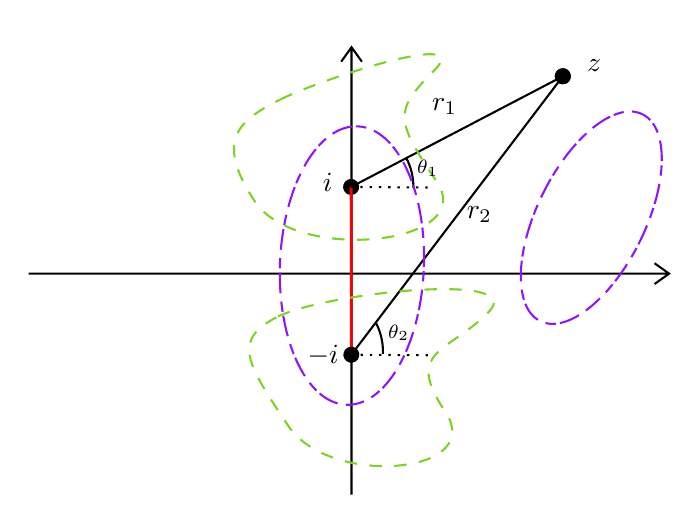
\begin{tikzpicture}[x=0.75pt,y=0.75pt,yscale=-1,xscale=1]
%uncomment if require: \path (0,300); %set diagram left start at 0, and has height of 300
% \begin{tikzpicture}[scale=1.0]

%Shape: Axis 2D [id:dp9226656499823862] 
\draw  (155.76,151.6) -- (464.29,151.6)(311.29,42.51) -- (311.29,258.08) (457.29,146.6) -- (464.29,151.6) -- (457.29,156.6) (306.29,49.51) -- (311.29,42.51) -- (316.29,49.51)  ;
%Straight Lines [id:da6217297407330797] 
\draw    (311.09,109.84) -- (413.09,56.51) ;
\draw [shift={(413.09,56.51)}, rotate = 332.4] [color={rgb, 255:red, 0; green, 0; blue, 0 }  ][fill={rgb, 255:red, 0; green, 0; blue, 0 }  ][line width=0.75]      (0, 0) circle [x radius= 3.35, y radius= 3.35]   ;
\draw [shift={(311.09,109.84)}, rotate = 332.4] [color={rgb, 255:red, 0; green, 0; blue, 0 }  ][fill={rgb, 255:red, 0; green, 0; blue, 0 }  ][line width=0.75]      (0, 0) circle [x radius= 3.35, y radius= 3.35]   ;
%Straight Lines [id:da5187482795861946] 
\draw    (311.2,190.67) -- (413.09,56.51) ;

\draw [mark = +]   (311.09,109.84) -- (311.2,190.67) [color={rgb, 255:red, 255; green, 0; blue, 0 }  ][line width=1.0];

\draw [shift={(413.09,56.51)}, rotate = 307.22] [color={rgb, 255:red, 0; green, 0; blue, 0 }  ][fill={rgb, 255:red, 0; green, 0; blue, 0 }  ][line width=0.75]      (0, 0) circle [x radius= 3.35, y radius= 3.35]   ;
\draw [shift={(311.2,190.67)}, rotate = 307.22] [color={rgb, 255:red, 0; green, 0; blue, 0 }  ][fill={rgb, 255:red, 0; green, 0; blue, 0 }  ][line width=0.75]      (0, 0) circle [x radius= 3.35, y radius= 3.35]   ;

%Straight Lines [id:da04858347938757013] 
\draw [line width=0.75]  [dash pattern={on 0.84pt off 2.51pt}]  (311.2,190.67) -- (320.53,190.73) -- (349.2,190.93) ;
%Straight Lines [id:da03323421997367659] 
\draw [line width=0.75]  [dash pattern={on 0.84pt off 2.51pt}]  (311.09,109.84) -- (333.2,110) -- (349.09,110.11) ;
%Shape: Arc [id:dp3288057226479919] 
\draw  [draw opacity=0] (337.73,96.02) .. controls (339.88,100.15) and (341.09,104.85) .. (341.09,109.84) .. controls (341.09,109.98) and (341.09,110.12) .. (341.09,110.26) -- (311.09,109.84) -- cycle ; \draw   (337.73,96.02) .. controls (339.88,100.15) and (341.09,104.85) .. (341.09,109.84) .. controls (341.09,109.98) and (341.09,110.12) .. (341.09,110.26) ;  
%Shape: Arc [id:dp0808155872490477] 
\draw  [draw opacity=0] (323.18,175.58) .. controls (325.25,179.66) and (326.43,184.28) .. (326.43,189.17) .. controls (326.43,189.55) and (326.42,189.92) .. (326.41,190.29) -- (296.43,189.17) -- cycle ; \draw   (323.18,175.58) .. controls (325.25,179.66) and (326.43,184.28) .. (326.43,189.17) .. controls (326.43,189.55) and (326.42,189.92) .. (326.41,190.29) ;  
%Shape: Polygon Curved [id:ds972117629019259] 
\draw  [color={rgb, 255:red, 126; green, 211; blue, 33 }  ,draw opacity=1 ][dash pattern={on 4.5pt off 4.5pt}][line width=0.75]  (277.2,67.6) .. controls (297.2,57.6) and (371.2,33.6) .. (351.2,53.6) .. controls (331.2,73.6) and (332.53,77.6) .. (352.53,107.6) .. controls (372.53,137.6) and (284.81,146.92) .. (264.81,116.92) .. controls (244.81,86.92) and (257.2,77.6) .. (277.2,67.6) -- cycle ;
%Shape: Polygon Curved [id:ds36093576999491384] 
\draw  [color={rgb, 255:red, 126; green, 211; blue, 33 }  ,draw opacity=1 ][dash pattern={on 4.5pt off 4.5pt}][line width=0.75]  (275.87,172.27) .. controls (298.53,160.93) and (397.2,150.27) .. (377.2,170.27) .. controls (357.2,190.27) and (336.53,188.27) .. (356.53,218.27) .. controls (376.53,248.27) and (300.81,254.92) .. (280.81,224.92) .. controls (260.81,194.92) and (253.2,183.6) .. (275.87,172.27) -- cycle ;
%Shape: Ellipse [id:dp5218651449001477] 
\draw  [color={rgb, 255:red, 144; green, 19; blue, 254 }  ,draw opacity=1 ][dash pattern={on 3.75pt off 3pt on 7.5pt off 1.5pt}] (313.49,214.35) .. controls (294.34,218.61) and (277.9,192.22) .. (276.79,155.41) .. controls (275.68,118.61) and (290.31,85.32) .. (309.47,81.07) .. controls (328.63,76.82) and (345.06,103.2) .. (346.17,140.01) .. controls (347.28,176.81) and (332.65,210.1) .. (313.49,214.35) -- cycle ;
%Shape: Ellipse [id:dp6256363959244384] 
\draw  [color={rgb, 255:red, 144; green, 19; blue, 254 }  ,draw opacity=1 ][dash pattern={on 3.75pt off 3pt on 7.5pt off 1.5pt}] (428.07,166.23) .. controls (409.33,182.7) and (393.58,177.43) .. (392.88,154.46) .. controls (392.19,131.49) and (406.82,99.52) .. (425.56,83.05) .. controls (444.3,66.58) and (460.05,71.85) .. (460.75,94.82) .. controls (461.44,117.79) and (446.81,149.76) .. (428.07,166.23) -- cycle ;


% Text Node
\draw (296,101.73) node [anchor=north west][inner sep=0.75pt]    {$i$};
% Text Node
\draw (288.67,184.4) node [anchor=north west][inner sep=0.75pt]    {$-i$};
% Text Node
\draw (423.33,47.07) node [anchor=north west][inner sep=0.75pt]    {$z$};
% Text Node
\draw (365.33,117.73) node [anchor=north west][inner sep=0.75pt]    {$r_{2}$};
% Text Node
\draw (348.67,65.73) node [anchor=north west][inner sep=0.75pt]    {$r_{1}$};
% Text Node
\draw (341.33,95.4) node [anchor=north west][inner sep=0.75pt]  [font=\scriptsize]  {$\theta _{1}$};
% Text Node
\draw (327.33,174.73) node [anchor=north west][inner sep=0.75pt]  [font=\scriptsize]  {$\theta _{2}$};


\end{tikzpicture}


    % \begin{tikzpicture}[scale=3]
    \draw[->] (-0.2,0) -- (1.2,0) node[right] {$\operatorname{Re}(z)$};
    \draw[->] (0,-0.2) -- (0,1.0) node[above] {$\operatorname{Im}(z)$};
    % \draw[dashed] (0.5,-1.5) -- (0.5,1.5);
    % \draw[dashed] (-1.5,0.5) -- (1.5,0.5);
    \draw[-latex] (1.0,0.3) -- (1.0,0.8) node[midway, right] {$\substack{\Delta y\to 0\\\Delta x=0}$};
    \draw[-latex] (0.3,0.8) -- (1.0,0.8) node[midway, above] {$\substack{\Delta x\to 0\\\Delta y=0}$};
    \filldraw [fill=none] (1,0.8) circle (0.02) node[above right] {$z_0$};
    \node at (0,0) [below left] {$O$};
\end{tikzpicture}
    \caption{对函数$f(z) = \sqrt{z^2 + 1}$的路径选取和割线示意图.}
    \label{fig:contours}
\end{figure}

\begin{example}
找出函数$f(z) = \sqrt{z^2 + 1}$的支点,并取合适的割线.
\end{example}
\begin{solution}
不难看出,
\[
  f(z) = \sqrt{z + \imath} \sqrt{z-\imath} .
\]
前面我们了解了$f(z)=\sqrt{z}$的支点为$z=0$,不难看出来,$z=\pm \imath$也会成为
该函数的两个支点.
如图\ref{fig:contours}所示,令
\[ z - i = r_1 e^{\imath \theta_1 } \quad 
    z + i = r_2 e^{\imath \theta 2}
\]
我们有\[f(z) = \sqrt{r_1 r_2} e^{\imath \half (\theta_1 + \theta_2)}.\]
如果我们做以下几种情况的闭合路径$C$,我们会得到不同的情况.若$C$
\begin{enumerate}
    \item[(i)] 不包含两个支点,那么$\theta_1 \to \theta_1, \theta_2 \to \theta_2$, 于是$f(z)\to f(z)$;
    \item[(ii)] 包含$\imath$但不含$-\imath$,那么$\theta_1 \to \theta_1 + 2\pi, \theta_2 \to \theta_2$, 于是$f(z)\to - f(z)$;
    \item[(iii)] 包含$-\imath$但不含$\imath$,那么$\theta_1 \to \theta_1, \theta_2 \to \theta_2  + 2\pi$, 于是$f(z)\to - f(z)$;
    \item[(iv)] 包含$\pm \imath$两个支点,那么$\theta_1 \to \theta_1  + 2\pi, \theta_2 \to \theta_2  + 2\pi$, 于是$f(z)\to  f(z)$.
\end{enumerate}
因此,为了阻止闭合路径绕支点完成完整的回路,我们必须选择合适的割线.图中连接$\pm \imath$的标红线段是一种选择.
\end{solution}

\section{复变函数积分}
\subsection[定义和性质]{复变函数的积分}
有了复变函数微分的基础,我们现在来讨论积分。复变函数的积分的定义可以同实变函数积分的类比得到。
在复平面上取一个路径$\ell$,起终点为$A(z_0),B(z_n)$,沿着该路径定义了一连续函数$f(z)$,用$n-1$个点$z_1, z_2,\cdot, z_{n-1}$将该路径
$\ell$分成$n$个线段(见图\ref{fig:complex_integral})。函数$f(z)$在线段$z_{k-1}\rightarrow z_{k}$上任意一点$\xi_k$的值乘上线段的长度$\Delta z_k = z_k - z_{k-1}$并求和,即
\begin{equation}
    S_n = \sum_{k=1}^{n} f(\xi_k) (z_{k} - z_{k-1}) .
\end{equation}
\begin{figure}[htbp]
    \centering
    % \begin{tikzpicture}[scale=1.5]

%     % 绘制坐标轴
%     \draw[->] (-0.5,0) -- (2.5,0) node[right] {$\Re$};
%     \draw[->] (0,-1.5) -- (0,2.5) node[above] {$\Im$};
    
%     % 定义积分路径的控制点
%     \coordinate (A) at (0.4,0.8);
%     \coordinate (B) at (1.5,1.2);
%     \coordinate (C) at (2,0.5);
%     \coordinate (D) at (1.2,-0.5);
    
%     % 绘制复平面上的积分路径
%     % \draw[thick, red] (0,0) -- (A) .. controls (B) .. (C) -- (D) -- (0,0);
%     % \draw[thick, red] (0,0) -- (A) .. controls (B) .. (C) -- (D) .. (0,0);
    
%     % 贝叶斯曲线参数
%     \def\a{-0.5}
%     \def\b{-1}
%     \def\c{0}
%     \def\d{0.5}
%     % 绘制贝叶斯曲线
%     % \draw[thick, blue] plot[domain=-1:2, samples=100] (\x, {\a + \b * exp(-(\x - \c)^2 / (2 * \d^2))});

%     \draw[thick, blue] plot[domain=0.5:2, samples=100] (\x, {\a + \b * \x + \c * \x^2 + \d * \x^3});

%     % 绘制复平面上的积分路径标记
%     % \node[black, above right] at (A) {$z_1$};
%     % \node[black, above] at (B) {$z_2$};
%     % \node[black, above right] at (C) {$z_3$};
%     % \node[black, below right] at (D) {$z_4$};
    
%     % 绘制复平面上的积分起点和终点
%     \filldraw[black] (0,0) circle (0.03) node[below left] {$O$};
%     \filldraw[black] (1.2,-0.5) circle (0.03) node[below right] {$z$};
    
%     % 绘制复平面上的积分路径标记
%     % \draw (0.8,1) node {$\Gamma$};
    
%     \end{tikzpicture}








\tikzset{every picture/.style={line width=0.75pt}} %set default line width to 0.75pt        

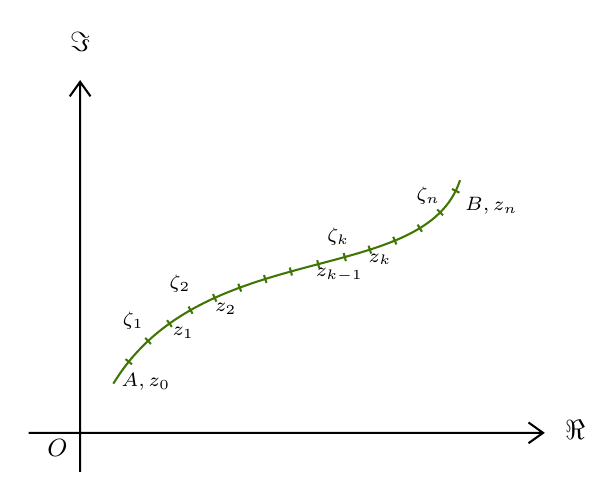
\begin{tikzpicture}[x=0.75pt,y=0.75pt,yscale=-1,xscale=1]
%uncomment if require: \path (0,300); %set diagram left start at 0, and has height of 300

%Shape: Axis 2D [id:dp2198947180733517] 
\draw  (83,214.11) -- (330.8,214.11)(107.78,45) -- (107.78,232.9) (323.8,209.11) -- (330.8,214.11) -- (323.8,219.11) (102.78,52) -- (107.78,45) -- (112.78,52)  ;
%Curve Lines [id:da014028466733404077] 
\draw [color={rgb, 255:red, 65; green, 117; blue, 5 }  ,draw opacity=1 ]   (123.8,190.4) .. controls (123.44,190.89) and (125,188.45) .. (125.62,187.51) .. controls (169.74,120.08) and (274.04,143.68) .. (290.8,92.4)(129.64,178.59) -- (132.75,181.1)(139.15,168.38) -- (141.88,171.31)(149.65,159.83) -- (151.98,163.08)(159.97,153.25) -- (161.95,156.73)(171.78,147.26) -- (173.43,150.9)(183.98,142.28) -- (185.36,146.03)(196.37,138.08) -- (197.56,141.9)(208.77,134.45) -- (209.84,138.3)(221.98,130.9) -- (223,134.77)(234.73,127.48) -- (235.79,131.34)(246.75,123.93) -- (247.97,127.74)(258.61,119.66) -- (260.14,123.35)(270.38,113.8) -- (272.46,117.22)(279.82,106.5) -- (282.65,109.33)(286.93,96.63) -- (290.52,98.4) ;

% Text Node
\draw (90.5,215.9) node [anchor=north west][inner sep=0.75pt]  [font=\small]  {$O$};
% Text Node
\draw (340,206.4) node [anchor=north west][inner sep=0.75pt]    {$\Re $};
% Text Node
\draw (101.5,19.4) node [anchor=north west][inner sep=0.75pt]    {$\Im $};
% Text Node
\draw (126.3,183.8) node [anchor=north west][inner sep=0.75pt]  [font=\scriptsize]  {$A,z_{0}$};
% Text Node
\draw (245.3,126.3) node [anchor=north west][inner sep=0.75pt]  [font=\scriptsize]  {$z_{k}$};
% Text Node
\draw (219.8,133.3) node [anchor=north west][inner sep=0.75pt]  [font=\scriptsize]  {$z_{k-1}$};
% Text Node
\draw (171.3,150.3) node [anchor=north west][inner sep=0.75pt]  [font=\scriptsize]  {$z_{2}$};
% Text Node
\draw (126.8,154.3) node [anchor=north west][inner sep=0.75pt]  [font=\scriptsize]  {$\zeta _{1}$};
% Text Node
\draw (150.8,161.8) node [anchor=north west][inner sep=0.75pt]  [font=\scriptsize]  {$z_{1}$};
% Text Node
\draw (291.8,99.3) node [anchor=north west][inner sep=0.75pt]  [font=\scriptsize]  {$B,z_{n}$};
% Text Node
\draw (149.3,136.8) node [anchor=north west][inner sep=0.75pt]  [font=\scriptsize]  {$\zeta _{2}$};
% Text Node
\draw (225.3,113.8) node [anchor=north west][inner sep=0.75pt]  [font=\scriptsize]  {$\zeta _{k}$};
% Text Node
\draw (268.3,94.3) node [anchor=north west][inner sep=0.75pt]  [font=\scriptsize]  {$\zeta _{n}$};


\end{tikzpicture}


    \caption{复变函数积分示意图。光滑曲线$\ell$上取一系列点$z_k$将其分成$n$小段。}
    \label{fig:complex_integral}
\end{figure}
当$n\to \infty$, 求和则转化为积分。当这个和的极限存在且
与$\xi_k$的选取无关时,这个极限称为
函数$f(z)$沿着路径$\ell$的\textbf{路径积分}(Contour integral), 记作
$\int_{\ell} f(z) dz$,即
\begin{equation}
    \int_{\ell} f(z) dz = \lim_{n\to \infty} \sum_{i=k}^{n} f(\xi_k) (z_{k} - z_{k-1}) . 
\end{equation}
其实,我们还可以将该定义用实虚部的方式表达出来,
\begin{align}
    \int_{\ell} f(z) dz  & = \int_{\ell} \left( u(x,y) + \imath v(x,y) \right) (dx + \imath dy) 
    \\
    & = \int_{\ell} \left( u(x,y) dx  -  v(x,y) dy \right) + \imath \int_{\ell}  \left( v(x,y) dx  + u(x,y)dy \right) 
\end{align}
这样一来,复变函数的路径积分就转化成了两个实变函数的线积分。因此,很多实函数线积分的性质可以应用在路径积分上。



\subsection{柯西积分定理}
\label{subsec:cauchy_theorem}
柯西积分定理(简称柯西定理)说的是,如果$f(z)$是解析函数,$f'(z)$在闭合路径$C$%构成的单连通
区域内任一点连续,有
\begin{equation}
    \oint_C f(z) dz = 0.
\end{equation}
所有的闭合回路的积分我们用$\oint$来表示.证明会用到格林公式和柯西-黎曼条件,具体参考其他书目,其中
格林公式为
\begin{equation}
    \oint_\ell P dx + Q dy = \iint_S \left( \frac{\partial Q}{\partial x} - \frac{\partial P}{\partial y}  \right) dx dy
\end{equation}
对于某些区域有奇点的情况,我们可以取一绕过奇点的闭合路径,如图\ref{fig:complexregion}所示的情况.柯西定理重要的应用在于将沿某一路径积分转化为
另一个或多个路径积分的求和.通常这样来规定正方向,当观察者沿着该方向前进时,区域总是在观察者的左侧.
\begin{figure}
    \centering
    

\tikzset{every picture/.style={line width=0.75pt}} %set default line width to 0.75pt        

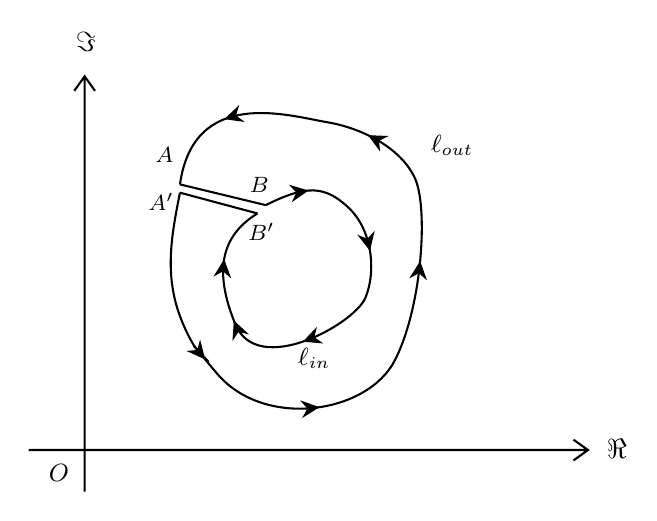
\begin{tikzpicture}[x=0.75pt,y=0.75pt,yscale=-1,xscale=1]
%uncomment if require: \path (0,300); %set diagram left start at 0, and has height of 300

%Shape: Axis 2D [id:dp04611299520330148] 
\draw  (107,219.06) -- (376.47,219.06)(133.95,39) -- (133.95,239.07) (369.47,214.06) -- (376.47,219.06) -- (369.47,224.06) (128.95,46) -- (133.95,39) -- (138.95,46)  ;
%Curve Lines [id:da4408212979573587] 
\draw    (179.87,91.07) .. controls (186.53,43.73) and (232.62,58.07) .. (250.53,61.07) .. controls (268.45,64.07) and (286.87,74.07) .. (293.2,88.4) .. controls (299.53,102.73) and (296.53,150.4) .. (283.33,175.97) .. controls (270.13,201.54) and (220.5,209.23) .. (197.65,182.12) .. controls (174.81,155.01) and (194.63,178.2) .. (193.33,175.97) ;
\draw [shift={(201.24,59.65)}, rotate = 342.17] [fill={rgb, 255:red, 0; green, 0; blue, 0 }  ][line width=0.08]  [draw opacity=0] (8.93,-4.29) -- (0,0) -- (8.93,4.29) -- (5.93,0) -- cycle    ;
\draw [shift={(270.48,67.37)}, rotate = 27.92] [fill={rgb, 255:red, 0; green, 0; blue, 0 }  ][line width=0.08]  [draw opacity=0] (8.93,-4.29) -- (0,0) -- (8.93,4.29) -- (5.93,0) -- cycle    ;
\draw [shift={(295.59,127.97)}, rotate = 96.21] [fill={rgb, 255:red, 0; green, 0; blue, 0 }  ][line width=0.08]  [draw opacity=0] (8.93,-4.29) -- (0,0) -- (8.93,4.29) -- (5.93,0) -- cycle    ;
\draw [shift={(247.14,198.42)}, rotate = 173.71] [fill={rgb, 255:red, 0; green, 0; blue, 0 }  ][line width=0.08]  [draw opacity=0] (8.93,-4.29) -- (0,0) -- (8.93,4.29) -- (5.93,0) -- cycle    ;
\draw [shift={(192.02,175.42)}, rotate = 230.07] [fill={rgb, 255:red, 0; green, 0; blue, 0 }  ][line width=0.08]  [draw opacity=0] (8.93,-4.29) -- (0,0) -- (8.93,4.29) -- (5.93,0) -- cycle    ;
%Straight Lines [id:da2752936846063838] 
\draw    (179.87,91.07) -- (221.2,101.07) ;
%Curve Lines [id:da2227786948358368] 
\draw    (221.2,101.07) .. controls (241.2,91.07) and (249.87,91.73) .. (261.2,102.4) .. controls (272.53,113.07) and (274.53,133.07) .. (269.2,145.73) .. controls (263.87,158.4) and (217.2,184.4) .. (206.53,158.4) .. controls (206.05,157.22) and (205.59,156.05) .. (205.17,154.91) .. controls (196.26,130.89) and (200.66,115.25) .. (217.2,105.07) ;
\draw [shift={(241.83,94.03)}, rotate = 170.78] [fill={rgb, 255:red, 0; green, 0; blue, 0 }  ][line width=0.08]  [draw opacity=0] (8.93,-4.29) -- (0,0) -- (8.93,4.29) -- (5.93,0) -- cycle    ;
\draw [shift={(271.41,123.08)}, rotate = 257.51] [fill={rgb, 255:red, 0; green, 0; blue, 0 }  ][line width=0.08]  [draw opacity=0] (8.93,-4.29) -- (0,0) -- (8.93,4.29) -- (5.93,0) -- cycle    ;
\draw [shift={(239.05,166.85)}, rotate = 339.24] [fill={rgb, 255:red, 0; green, 0; blue, 0 }  ][line width=0.08]  [draw opacity=0] (8.93,-4.29) -- (0,0) -- (8.93,4.29) -- (5.93,0) -- cycle    ;
\draw [shift={(205.83,156.66)}, rotate = 68.16] [fill={rgb, 255:red, 0; green, 0; blue, 0 }  ][line width=0.08]  [draw opacity=0] (8.93,-4.29) -- (0,0) -- (8.93,4.29) -- (5.93,0) -- cycle    ;
\draw [shift={(201.16,127.05)}, rotate = 95.63] [fill={rgb, 255:red, 0; green, 0; blue, 0 }  ][line width=0.08]  [draw opacity=0] (8.93,-4.29) -- (0,0) -- (8.93,4.29) -- (5.93,0) -- cycle    ;
%Straight Lines [id:da5896769090029934] 
\draw    (179.87,95.07) -- (217.2,105.07) ;
%Curve Lines [id:da07734592378285976] 
\draw    (187.2,169.73) .. controls (171.07,142.83) and (174.53,121.73) .. (179.87,95.07) ;

% Text Node
\draw (115.17,224.57) node [anchor=north west][inner sep=0.75pt]  [font=\small]  {$O$};
% Text Node
\draw (299.33,66.07) node [anchor=north west][inner sep=0.75pt]  [font=\small]  {$\ell _{out}$};
% Text Node
\draw (166.67,71.73) node [anchor=north west][inner sep=0.75pt]  [font=\footnotesize]  {$A$};
% Text Node
\draw (211.33,108.4) node [anchor=north west][inner sep=0.75pt]  [font=\footnotesize]  {$B'$};
% Text Node
\draw (212,86.4) node [anchor=north west][inner sep=0.75pt]  [font=\footnotesize]  {$B$};
% Text Node
\draw (163.33,93.73) node [anchor=north west][inner sep=0.75pt]  [font=\footnotesize]  {$A'$};
% Text Node
\draw (235.33,168.73) node [anchor=north west][inner sep=0.75pt]  [font=\small]  {$\ell _{in}$};
% Text Node
\draw (128.17,16.07) node [anchor=north west][inner sep=0.75pt]    {$\Im $};
% Text Node
\draw (384,212.4) node [anchor=north west][inner sep=0.75pt]    {$\Re $};


\end{tikzpicture}

    \caption{复杂路径示意图.}
    \label{fig:complexregion}
\end{figure}
由于$\ell_{in}$和$\ell_{out}$与割线$AB,A'B'$组成了闭合回路,根据柯西定理,我们有
\[
    \left[ \oint _{\ell_{out}} + \int _{\ell_{AB}} + \oint _{\ell_{in}} + \int _{\ell_{B'A'}} \right] f(z) dz = 0 .
\]   
由于割线$AB$与$A'B'$可以无限接近,可以看出二者方向相反,这两项互相抵消.于是我们有
\[
    \left[ \oint _{\ell_{out}} + \oint _{\ell_{in}}  \right] f(z) dz = 0,
\]
即
\[
    \oint_{\ell_{out}} f(z) dz = - \oint _{\ell_{in}}f(z) dz .
\]
若用逆时针方向积分表示,并考虑多个内边界$\ell_{i}$,我们有
\begin{equation}
    \ointctrclockwise_{\ell_{out}} f(z) dz = \sum_{i=1}^{n} \ointctrclockwise_{\ell_{in}} f(z) dz .
\end{equation}
就是说,外边界逆时针方向积分等于所有内边界逆时针方向积分之和.只要积分起点和终点固定,当积分路径连续变形时(即不跳过奇点),函数的积分值不变.

下面给出一个重要的例题.
\begin{example}
计算积分\[ I = \oint_\ell (z-\alpha)^n dz, \]其中$n$为整数.
\end{example}
\begin{solution}
首先,有柯西定理易知,若回路$\ell$不包含$\alpha$,则被积函数在$\ell$所围区域上是解析的,故积分值为零.下面讨论$\ell$包围$\alpha$的情形.
如果$n\geq 0$,被积函数在$\ell$所围区域是解析的,积分为零.若$n<0$,则有一个奇点$\alpha$.取以$\alpha$为圆心半径为$R$的圆周$C$,$R$大小任意.
于是圆周上有$z-\alpha = Re^{\imath \theta}$.
$$
\begin{aligned}
    I &= \oint_\ell (z-\alpha)^n dz\\
     &= \oint_c R^n e^{\imath n \theta} d (\alpha + R e^{\imath \theta})\\
     & =  \imath R^{n+1} \int_0^{2\pi} e^{\imath (n+1)\theta}  d\theta \\
     & = 0 \quad \textrm{if} \quad n\neq -1.
\end{aligned}
$$

当$n = -1$时, $I = 2\pi \imath$.其实,从原函数的角度来看,这个结果很容易理解.当$n\neq -1$,原函数为$(z-\alpha)^{n+1}/(n+1)$, 绕$\alpha$一周
原函数变化量为零.而当$n=-1$时,原函数时$\ln(z-\alpha)$, 绕一周变化量为$2\pi \imath$.因此我们得到了非常重要的表达式
$$
    \begin{aligned}
        & \frac{1}{2 \pi \imath} \oint_l \frac{d z}{z-\alpha}= \begin{cases}0 & (l \text { 不包围 } \alpha), \\
        1 & (l \text { 包围 } \alpha) . \end{cases} \\
        & \frac{1}{2 \pi \imath} \oint_l(z-\alpha)^n d z=0 \quad(n \neq-1) .
        \end{aligned}
$$
\end{solution}
\subsection{柯西积分公式}
\label{subsec:cauchy_formula}
复变函数理论中最重要的一个公式是柯西积分公式.若$f(z)$在一闭合回路围成的区域内解析,$z_0$为区域内一点,
则有
\begin{equation}
    f\left(z_0\right)=\frac{1}{2 \pi i} \oint_C \frac{f(z)}{z-z_0} d z .  
\end{equation}
柯西公式将解析函数在任何一内点 $z_0$ 的值 $f(z_0)$ 用沿边界线 $l$ 的回路积分 表示了出来.
也就是说,一个解析函数在闭合回路$C$内任意点$z_0$的值完全由该路径上的值决定的. 
这看起来不可思议,但又是必然结果.从物理上说, 解析函数紧密联系于平面标量场, 而平面场的边界条件决定着区域内部的场.
我们可以通过前面提到的柯西定理来证明.我们需要围绕$z_0$选取一个半径为$r$的内圆$\gamma$,由于$f(z)/(z-z_0)$在
内圆与$C$形成的区域解析,故我们有
\[ \frac{1}{2 \pi \imath} \oint_C \frac{f(z)}{z-z_0} d z = \frac{1}{2 \pi \imath} \oint_\gamma \frac{f(z)}{z-z_0} d z
    \]
有$z-z_0 = re^{\imath \theta}$,于是
\begin{equation}
    \begin{aligned}
        I &= \oint_\gamma \frac{f(z)}{z-z_0} d z
        \\
        & = \int _0 ^{2\pi} \frac{f(z_0 + re^{\imath \theta})}{re^{\imath \theta}} ire^{\imath \theta} d\theta
        \\
        & = \imath \int _0 ^{2\pi} f(z_0 + re^{\imath \theta}) d\theta
    \end{aligned}
\end{equation}
现令内圆半径$r\to 0$,则有$I\to 2\pi\imath f(z_0)$,得证.
由于$z_0$的任意性,我们可以改写成$z$,而把积分变量改成$\zeta$,则有
\begin{equation}
    f(z) = \frac{1}{2\pi \imath} \oint_C \frac{f(\zeta)}{\zeta - z} d \zeta.
    \label{eq:cauchy_formula}
\end{equation}

对柯西公式\eqref{eq:cauchy_formula}求导,我们有
\begin{equation}
    f'(z) = \frac{1!}{2\pi \imath} \oint_C \frac{f(\zeta)}{(\zeta - z)^2} d \zeta.
    \label{eq:cauchy_formula_1st_derivative}
\end{equation}
反复求导则有
\begin{equation}
    f^{(n)}(z) = \frac{n!}{2\pi \imath} \oint_C \frac{f(\zeta)}{(\zeta - z)^{n+1}} d \zeta.
    \label{eq:cauchy_formula_nth_derivative}
\end{equation}
% 这是因为解析函数在各点的值通过柯西 - 黎曼方程相互联系着. 

下面介绍柯西公式的重要推论.

\textbf{模数原理} $f(z)$在闭区域上解析,$|f(z)|$只能在边界线上取极大值.

由$f(z)^n = \frac{1}{2\pi \imath} \oint_C \frac{f(\zeta)^n}{\zeta - z} d \zeta$,若$|f(\zeta)|$在$C$上极大值为$M$,
$|\zeta - z|$的极小值为$\delta$, $C$的长度为$s$,则
\[
  |f(z)|^n \leq \frac{1}{2\pi} \frac{M^n}{\delta} s  ,
\]
即
\[
    |f(z)| \leq M \left( \frac{s}{2\pi \delta} \right)^{\frac{1}{n}},
\]
令$n\to \infty$,$|f(z)| \leq M$.证毕.

\textbf{刘维尔(Liouville)定理} \quad 如$f(z)$在全平面上解析且有界,则$f(z)$必为常数.

\textbf{证} \quad $f$有界,即$|f(z)| \leq N$, 对$f'(z)$取模,取以$z$为圆心半径为$R$的圆周,可得
\[
  |f'(z)| \leq \frac{1}{2\pi} \frac{N} {R^2} 2\pi R = \frac{N}{R},
\]
由于$R$任意选定,令$R\to \infty$,有$f'(z) \equiv 0$,所以$f(z)$为常数.

刘维尔定理的一个应用是可以证明代数基本定理,即对任意$n$阶多项式(Polynomial)
\begin{equation}
    P(z) = \sum_{k=0}^{n} a_k z^k (n>0, a_n \neq 0)
    \label{eq:poly}
\end{equation}
有$n$个根满足$P(z) = 0$. 它的证明可以通过反证的方法. 假设$P(z)$没有零点,即$P(z)\neq 0$, 则$1/P(z)$是解析
且有界的,根据刘维尔定理可知$1/P(z)$为常数,即$P(z)$为常数,与$a_n\neq 0$矛盾.可以知道,$P(z)$至少有一个根,记为$\lambda_1$,
那么对$P(z)/(z-\lambda_1)$这一$n-1$阶多项式进行上述论证,我们可以降次直至一阶多项式,共计$n$个根,因此$n$阶多项式
有$n$个根.

\section{复数级数}
\subsection{级数的基本性质}
物理学和工程学中的一些函数常常可以用无穷级数来表示。一个很有用的例子,
\begin{equation}
    1+ x + x^2 + x^3 + \cdots = \frac{1}{1-x} \textrm{。}
\end{equation}
有了该式,我们可以处理更复杂的级数,如
\begin{equation}
    1 + a \cos \theta + a^2 \cos 2\theta + a^3 \cos 3\theta + \cdots = ? 
\end{equation}
有了前面的复数概念,我们有
\begin{equation}
    \cos \theta = \Re e^{\imath \theta} = \frac{e^{\imath \theta} +e^{-\imath \theta} }{2} \textrm{。}
\end{equation}
于是,
\begin{align*}
   & 1 + a \cos \theta + a^2 \cos 2\theta + a^3 \cos 3\theta + \cdots 
    \\  
 = &  1 + \half a e^{\imath \theta} + \half a e^{- \imath \theta} + \half a^2 e^{2\imath \theta} + \half a^2 e^{-2\imath \theta}  + \cdots 
 \\  
 =   & \half \left( 1 + a e^{\imath \theta} + a^2 e^{2\imath \theta} + \cdots \right)  
+ \half \left( 1 + a e^{- \imath \theta} + a^2 e^{-2\imath \theta}  + \cdots \right) 
\\  
= &  \half \frac{1}{1 - a e^{\imath \theta} } + \half \frac{1}{1 - a e^{-\imath \theta} }
\\  
= &  \half \left[ \frac{1-a\cos\theta + \imath a \sin \theta }{(1-a\cos\theta)^2 + (a\sin \theta)^2} + \frac{1-a\cos\theta - \imath a \sin \theta}{(1-a\cos\theta)^2 + (a\sin \theta)^2} \right]
 \\  
= &  \frac{1-a\cos\theta}{1-2 a \cos\theta + a^2} \textrm{。}
\end{align*}
现在我们要处理一个稍微复杂的级数,
\begin{equation}
    S(x) = 1 - \frac{x}{2} + \frac{x^2}{3} - \frac{x^3}{4} + \cdots
\end{equation}
为了将上式化简,我们需要把它转换成一个我们熟知的形式。由于分母比较特殊,我们想办法摆脱这些数字。为此,我们对$x S(x)$求导,得到
\begin{align}
    \frac{d}{dx} ( x S(x))  &=   \frac{d}{dx} \left( x- \frac{x^2}{2} + \frac{x^3}{3} - \frac{x^4}{4} \right)
    \nonumber \\ 
    &= 1 - x^2 + x^3 - x^4 + \cdots 
    \nonumber \\ 
    & = \frac{1}{1+x} \,
\end{align}
于是我们有,$
    x S(x) = \ln (1 + x) + C \textrm{。}$
当$x=0$, $S(x) = 1, \ln (1+x) = 0$, 有$C=0$。最终我们得到了
\begin{equation}
    \ln (1+x) = x -  \frac{x^2}{2} + \frac{x^3}{3} - \frac{x^4}{4} = \sum_{k=1}^{\infty} \frac{(-1)^{k+1} x^k}{k} \textrm{。}
\end{equation}
我们还可以利用指数的级数表示
\begin{equation}
    e^{x} = \sum_{n=0}^{\infty} \frac{x^n}{n!} = 1 + \frac{x}{1} + \frac{x^2}{2} + \frac{x^3}{3} + \cdots 
\end{equation}
来求解正余弦函数的级数表示。
\begin{enumerate}
    \item 几何级数: $ 1 + x + x^2 + x^3 + \cdots + x^n$, 对$|x|<1$,收敛于$\frac{1}{1-x}$。
    \item 调和级数: $ 1 + \half + \frac{1}{3} + \cdot +\frac{1}{k} = \sum_{k=1} \frac{1}{k}$,发散。
\end{enumerate}

值得注意的是,以上的求和表示实际上假定了$|x|<1$这个条件。容易验证,$|x|\geq 1$,级数是发散的。一般的,我们将复数的概念拓展到级数,
\begin{equation}
    s_n = \sum_{k=1}^{n} w_{k}
\end{equation}
随着,$n\to \infty$,部分求和趋于一个定值$S$,即
\begin{equation}
    \lim_{n\to \infty} s_n = S \textrm{,}
\end{equation}
我们称无穷级数 $\sum_{k=1}^{n} w_{k}${\bf 收敛}并趋于$S$。如果级数的求和趋于$\pm \infty$,级数{\bf 发散}。对于如
\begin{equation}
    \sum_{k=1}^{\infty} (-1)^k = 1 - 1 + 1 - 1 \cdots 
\end{equation}
这样的级数取值在$\pm 1$之间振荡,我们也称其发散。级数收敛的必要条件很显然是$\lim_{k\to \infty} w_k = 0$。对于级数是否收敛,在什么条件下收敛显得十分重要。
对级数收敛的充分条件寻找,派生出了各种各样的判据。

\subsection{级数的收敛判定法}

\subsubsection{柯西判据}
柯西判据(Cauchy criterion)说的是,对于$\epsilon>0$, 总存在固定的$N$使得$|s_j - s_i|< \epsilon$, 其中$i,j$是任意大于$N$的整数.也就是说,若$j>i$,
\begin{equation}
    | w_{i+1} + w_{i+2} + \cdots + w_{j} | < \epsilon ,
\end{equation}
直观地理解,也就是说某项以后的所有求和可以忽略不计,即部分求和趋于某一值,级数收敛.对于复数项级数,一样成立.如果将复数项级数的每一项都取模组成新的级数,
记为
\begin{equation}
    \sum_{k=1} |w_k| = \sum_{k=1}\sqrt { u_k^2 + v_k^2},
\end{equation}
若该级数收敛,则称原级数\textbf{绝对收敛}.绝对收敛的级数必然是收敛的.如果级数收敛,但非绝对收敛,那么我们称它为\textbf{条件收敛}.
\subsubsection{比较判定法}
如果我们有某一已知正项级数 $\sum_k a_k$收敛,若级数的每一项都满足 $0 \leq w_k \leq a_k$, 那么可以判定$\sum_k w_k$收敛.
这可以利用柯西判据进行证明.相反的, 若同发散级数$\sum_{k} a_k$比较有,$0 \leq a_k  \leq w_k$, 那么可以判定$\sum_k w_k$发散.
对于复数项级数,比较判据可以表示为$0 \leq |w_k| \leq a_k$.

\begin{examplebox}{试判定级数$\sum_{k=1} k^{-p}, p\leq 1$收敛还是发散.}
    已知调和级数$\sum_{k=1}1/k$是发散的,而 $k^{-p} > k^{-1}$, 根据比较判定法,可知该级数发散.
\end{examplebox}

\subsubsection{达朗贝尔判据}
% 级数$\sum_{n} w_n$,对足够大的$N$和与$N$无关的常数$r$,若满足条件$w_{n+1} / w_{n} \leq r < 1$,那么该级数收敛.反之,若$w_{n+1} / w_{n} \geq >= 1$,
% ,该级数发散.
达朗贝尔方法又称比值判定法(D'Alembert Ratio Criterion).
若任意项级数 $\sum_{n=1}^{\infty} w_n$ 通项满足:
$$
\lim _{n \to \infty}\left|\frac{w_{n+1}}{w_n}\right|=q ,
$$
\begin{enumerate}
    \item 当 $q<1$ 时, 级数绝对收敛;
    \item 当 $q>1$ 时, 级数发散;
    \item 当 $q=1$ 时, 此方法无效,需要其他方法判定.
\end{enumerate}

\begin{examplebox}{试判断级数$\sum_{k=1} k/2^k$的收敛性.}
    利用比值判定法
    \[ 
        \lim_{k\to \infty} \frac{w_{k+1}}{w_k}=\lim_{k\to \infty} \frac{k+1}{2^{k+1}} / \frac{k}{2^{k}}=\frac{1}{2} 
        = \lim_{k\to \infty} \frac{1}{2}\left(1+\frac{1}{k}\right) 
        = \half < 1
    \]
    可见该级数是收敛的.
\end{examplebox}
% $\frac{w_{k+1}}{w_k}=r , r 5 k$ 死关,
% 世東 $r<1$ ,那昍数收斂.
% 当 $r=1$ ,榇弅
% $$
% \frac{a_{k+1}}{a_k}=\frac{k}{k+1}<
% $$
% $$
% \begin{gathered}
% \frac{w_{k+1}}{w_k}=\frac{k+1}{2^{k+1}} / \frac{k}{2^{k+}}=\frac{1}{2} \frac{k+1}{k} \Rightarrow \frac{1}{2}<1 \\
% =\frac{1}{2}\left(1+\frac{1}{k}\right) \leqslant \frac{3}{4} \quad(k \geqslant 2)
% \end{gathered}
% $$

% \subsubsection{莱布尼兹判据(Leibniz Criterion)}
此外,还有很多其他判定方法,如对于交错级数可以利用莱布尼兹判据(Leibniz Criterion).
% \begin{enumerate}
%     \item 
% \end{enumerate}

\subsection{幂级数(Power Series)}
本讲专门讨论在函数项级数中非常重要的一类级数,叫做幂级数。幂级数的各项都是幂函数,
\begin{equation}
    \sum_{k=0}^{\infty} a_k\left(z-z_0\right)^k=a_0+a_1\left(z-z_0\right)+a_2\left(z-z_0\right)^2+\cdots
\end{equation}
其中$z_0, a_i$都是复常数。这样的级数称为以 $z_0$ 为中心的幂级数。
该幂级数可能收敛,也可能发散。如果幂级数是收敛的,称$z_0$为该级数的\textbf{收敛点};反之若它是发散的,称$z_0$为该级数的\textbf{发散点}。
函数项级数式的所有收敛点的集合称为其\textbf{收敛域},所有发散点的集合称为其\textbf{发散域}。

现在利用达朗贝尔比值判定法,如果
\begin{equation}
    \lim _{k \rightarrow \infty} \frac{\left|a_{k+1}\right|\left|z-z_0\right|^{k+1}}{\left|a_k\right|\left|z-z_0\right|^k}
    =\lim _{k \rightarrow \infty}\left|\frac{a_{k+1}}{a_k}\right|\left|z-z_0\right|<1
\end{equation}
则级数绝对收敛。若记
\begin{equation}
    \lim_{k \rightarrow \infty} \left|\frac{a_{k+1}}{a_k}\right| = R^{-1},
\end{equation}
那么当$|z-z_0| < R$时,级数绝对收敛。若$|z-z_0| > R$时, 级数的模越来越大,级数发散。对于$|z-z_0| = R$的时候,无法简单判定。
例如幂级数$\sum_{k=0} \frac{1}{k} |z-z_0|^k$,可知$R=1$。$|z-z_0|=1$有两种情况:当$z-z_0 = +1$时, 由调和级数知道,该级数发散;而
当$z-z_0 = -1$时,由莱布尼兹判定法可知该级数收敛。

以$z_0$ 为圆心作一个半径为$R$的圆$C_R$。幂级数在圆的内部绝对收敛, 在圆外发散. 这个圆因而称为幂级数的\textbf{收敛圆}, 
它的半径则称为\textbf{收敛半径}。至于在收敛圆周上的收敛情况则需要具体分析。

\begin{examplebox}{求幂级数$1 - z^2 + z^4 - z^6\cdots$的收敛圆,$z$为复变数。}
    将$z^2$记作$t$,则本例的级数化成$1-t + t^2 - t^3\cdots$。系数$a_k =(-1)^k$, 因此t平面上收敛半径$R=1$。 
    因此$z$平面上收敛半径为$\sqrt{R}=1$。
\end{examplebox}
\subsection{泰勒级数(Taylor Series)和洛朗级数(Laurent Series)}
\label{subsec:taylor_laurent_series}
同实变函数泰勒级数展开一样,复变函数中解析函数自然也可以展为复变项的\textbf{泰勒级数}(Taylor series).
若$f(z)$在以$z_0$为圆心半径为$R$的圆$C_R$内(含圆上)解析,对圆内任意$z$,$f(z)$可以展为
\begin{equation}
    f(z) = \sum_{k=0}^{\infty} a_k (z-z_0)^k,
\end{equation}
其中
\begin{equation}
    a_k=\frac{1}{2 \pi \imath} \oint_{C_{R}} \frac{f(\zeta)}{\left(\zeta-z_0\right)^{k+1}} d \zeta
    =\frac{f^{(k)}\left(z_0\right)}{k !} ,
\end{equation}
且该展开唯一.

以上的证明如下.利用$1/(\zeta -z)$围绕$z_0$为圆心的几何级数,构造
\[
\frac{1}{\zeta -z} = \frac{1}{(\zeta -z_0) - (z - z_0)} = \frac{1}{\zeta - z_0}\frac{1}{ 1 - \frac{z-z_0}{\zeta - z_0}}
 = \sum_{k=0}^{\infty}\frac{(z-z_0)^k}{(\zeta - z_0)^{k+1}}.    
\]
将上式带入柯西公式有
\begin{equation}
    \begin{aligned}
        f(z) &= \frac{1}{2\pi \imath} \oint_C \frac{f(\zeta)}{\zeta - z} d \zeta
        \\
        &= \frac{1}{2\pi \imath} \sum_{k=0} ^{\infty} \oint_C \frac{f(\zeta)(z-z_0)^k}{(\zeta - z_0)^{k+1}} d \zeta
        \\
        &= \frac{1}{2\pi \imath} \sum_{k=0} ^{\infty}(z-z_0)^k 2\pi \imath \frac{f^{(k)}(z_0)}{k!}
        \\
        & = \sum_{k=0} ^{\infty}  \frac{f^{(k)}(z_0)}{k!} (z-z_0)^k
    \end{aligned}
\end{equation}
不难证明泰勒展开的唯一性.

以下是一个重要推论.若$f(z)$, $g(z)$在区域$R$解析,且在某些子区域$S\subset R$有$f(z)=g(z)$,那么全区域$R$内都有$f(z)=g(z)$.
该证明可通过构造$h(z) = f(z) - g(z)$然后利用该式在区域$R$内任意一点的的泰勒展开进行系数比较,可得$h(z)$在全区域内为零.
% \subsection{洛朗级数(Laurent Series)}
% \label{subsec:laurent_series}

\begin{examplebox}{在$z_0=1$的邻域上将$f(z) = \ln{z}$进行泰勒展开.}
    首先,$f(z) = \ln z $的支点为$0,\infty$.这里的展开中心为$z_0=1$非支点,各个单值分支互相独立.
    根据泰勒展开公式,我们需要将各个系数计算出来.
    \[
        \begin{array}{ll}
            f(z)=\ln z, & f(1)=\ln 1=n 2 \pi \imath \quad(n \text { 为整数 }) \text {; } \\
            f^{\prime}(z)=\frac{1}{z}, & f^{\prime}(1)=+1 ; \\
            f^{\prime \prime}(z)=-\frac{1 !}{z^2}, & f^{\prime \prime}(1)=-1 ! ; \\
            f^{(3)}(z)=\frac{2 !}{z^3}, & f^{(3)}(1)=+2 ! ; \\
            f^{(4)}(z)=-\frac{3 !}{z^4}, & f^{(4)}(1)=-3 ! ; \\
            \ldots & \cdots
            \end{array}
    \]
    于是,可以得到
    \[
    \ln z = 2 n \pi \imath + (z-1) - \frac{(z-1)^2}{2} +  \frac{(z-1)^3}{3} -  \frac{(z-1)^4}{4} \cdots
    \]
    按照比值判定法,该级数的收敛半径为$1$,需附加上$|z-1|< 1$这个收敛条件.我们称$n=0$的单值分支为$\ln z $的\textbf{主值}.
\end{examplebox}

目前为止,泰勒级数的展开的前提条件为区域内解析.然而,如果$f(z)$在区域内$z=z_0$的有奇点,那么泰勒展开就无法进行.假设$f(z)$仅在$z_0$有
一$p$阶\textbf{极点}(pole),其他区域均解析,我们有$g(z) = (z-z_0)^p f(z)$在区域内解析.因此,我们可以在$z_0$处进行泰勒展开
\begin{equation}
    g(z) = \sum_{k=0}^{\infty} b_k (z-z_0)^{k} .
\end{equation}
于是,我们可以将$f(z)$表示为
\begin{equation}
    f(z) = a_{-p} (z-z_0)^{-p} + \cdots a_{-1}(z-z_0)^{-1} + a_0 + a_{1} (z-z_0) + a_{2} (z-z_0)^2 + \cdots 
\end{equation}
作为泰勒级数的延伸,这样的级数我们称为\textbf{洛朗级数}(Laurent series).比较展开系数,不难得到$a_k = b_{k+p}$,
\begin{equation}
    a_k = b_{k+p} = \frac{1}{2\pi \imath} \oint \frac{g(\zeta)}{(\zeta - z_0)^{k+1+p}} d\zeta 
    = \frac{1}{2\pi \imath} \oint \frac{f(\zeta)}{(\zeta - z_0)^{k+1}} d\zeta
\end{equation}

洛朗级数所有幂次$k\geq 0$的项称为\textbf{解析部}(analytic part), 其余由$z-z_0$负幂次项称为\textbf{主部}(principal part).解析部的收敛半径记为
$R_1$.如果
主部收敛,那么对$|(z-z_0)^{-1}|$比某半径小的圆内收敛.若该圆半径为$1/R_2$,可以知当$|z-z_0|> R_2$,主部收敛.
如果$R_2 < R_1$那么级数在环域$R_2 < |z- z_0| < R_1$内绝对一致收敛,级数求和为解析函数,级数可以逐项求导.该环域称为\textbf{收敛环}.
如果$R_2 > R_1$那么该级数发散.

\begin{examplebox}{在$z_0 = 0$的邻域上将$e^{1/z}$展开.}
指数$e^z$的泰勒展开为
\[
    \mathrm{e}^z=\sum_{k=0}^{\infty} \frac{1}{k !} z^k=1+\frac{1}{1 !} z+\frac{1}{2 !} z^2+\frac{1}{3 !} z^3+\cdots \quad(|z|<\infty),    
\]
替换$z$成$1/z$得到
\[
    \mathrm{e}^{\frac{1}{z}}=\sum_{k=0}^{\infty} \frac{1}{k !} z^k=1+\frac{1}{1 !} \frac{1}{z}+\frac{1}{2 !} \frac{1}{z^2}+\frac{1}{3 !} \frac{1}{z^3}+\cdots \quad(|\frac{1}{z}|<\infty),    
\]
即有
\[
e^{\frac{1}{z}} = \sum_{k=-\infty}^{0} \frac{1}{(-k)!} z^k ( |z| > 0) .
\]
\end{examplebox}
% \subsection{洛郎级数(Laurent Series)}
\label{subsec:laurent_series}

\subsection{奇点的分类}
\label{subsec:singular_points}
\section{留数定理及应用}
\input{residue_theorem.tex}
\section{留数定理应用}
\subsection{三角函数的积分}
考虑积分区间为$\left[ 0, 2\pi \right]$,被积函数为三角函数有理式的积分
\begin{equation}
    \int_{0}^{2\pi} R(\cos{x}, \sin{x}) dx,
\end{equation}
当实变数 $x$ 从 0 变到 $2 \pi$ 时, 复变数 $z=e^{\imath x}$ 从 $z=1$ 出发沿单位圆 $|z|=1$ 逆时针 走一圈又回到 $z=1$,
实变定积分化为复变回路积分, 就可以应用留数定理了. 至于实变定积分里的 $\cos x, \sin x$ 和 $d x$, 作如下变换:
$$
\cos x=\frac{1}{2}\left(z+z^{-1}\right), \quad \sin x=\frac{1}{2 \imath}\left(z-z^{-1}\right), \quad d x=\frac{1}{\imath z} d z .
$$
于是, 原积分化为
$$
I=\oint_{|z|=1} R\left(\frac{z+z^{-1}}{2}, \frac{z-z^{-1}}{2 \imath}\right) \frac{d z}{\imath z}
$$
利用留数定理即可求得.

\begin{example}
求定积分\[I=\int_0^{2 \pi} \frac{d \theta}{1+a \cos \theta}, \quad|a|<1 \]
\end{example}
\begin{solution}
    根据上面的方法,可得
    \[
        \begin{aligned}
        I & =-\imath \oint_{|z|=1} \frac{d z}{z\left[1+(a / 2)\left(z+z^{-1}\right)\right]} \\
        & =-\imath \frac{2}{a} \oint \frac{d z}{z^2+(2 / a) z+1} .
        \end{aligned}
    \]
    两个极点分别为
    \[
        z_1=-\frac{1+\sqrt{1-a^2}}{a} \quad \text {和} \quad z_2=-\frac{1-\sqrt{1-a^2}}{a}
    \]
    不难看出,$z_1$在单位圆外,$z_2$在单位圆内.积分可以写成
    \[
      \oint \frac{dz}{(z-z_1)(z-z_2)}   
    \]
    留数则为$\frac{1}{z_2 - z_1}$, 利用留数定理可得 
    \[
      I=  -\imath \frac{2}{a} 2\pi\imath \frac{1}{z_2 - z_1} = \frac{2}{\sqrt{1 - a^2}} . 
    \]
\end{solution}



\subsection{积分上下限为$( -\infty, \infty)$}
 考虑如下形式的定积分
 \[
    \int_{-\infty}^{\infty} f(x) dx
 \]
 我们先讨论复变函数 $f(z)$ 在实轴上没有奇点的情况,有奇点的情况后面讨论. 
被积函数在上半平面除有限个奇点外是解析的; 当 $z$ 在上半平面及实轴上 $\to \infty$ 时, 
$z f(z)$ 一致地 $\to 0$.

取如图所示的上半平面的半径为$R$的半圆路径$\ell$.路径积分可以写成两部分的和
\begin{equation}
    \oint_l f(z) d z=\int_{-R}^R f(x) d x+\int_{C_R} f(z) d z .
\end{equation}
根据留数定理,上式等于$2\pi \imath  \sum_j \Res f(z_j)$.
%


\tikzset{every picture/.style={line width=0.75pt}} %set default line width to 0.75pt        

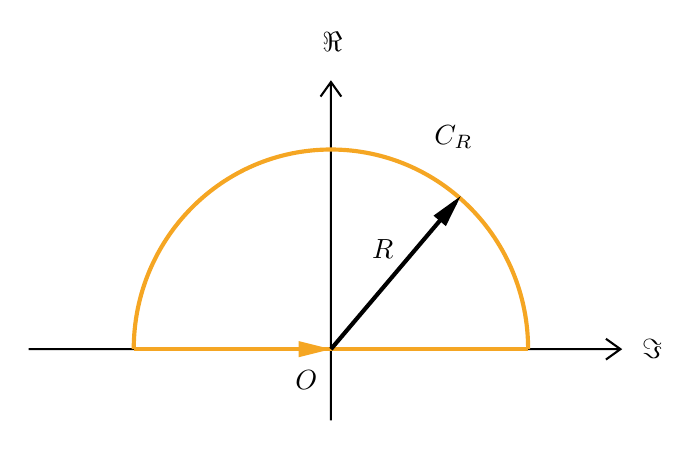
\begin{tikzpicture}[x=0.75pt,y=0.75pt,yscale=-1,xscale=1]
%uncomment if require: \path (0,266); %set diagram left start at 0, and has height of 266

%Shape: Axis 2D [id:dp1282392211894816] 
\draw  (162,181.79) -- (447.09,181.79)(307.61,53.09) -- (307.61,216.09) (440.09,176.79) -- (447.09,181.79) -- (440.09,186.79) (302.61,60.09) -- (307.61,53.09) -- (312.61,60.09)  ;
%Shape: Arc [id:dp1814309272431356] 
\draw  [draw opacity=0][line width=1.5]  (212.6,181.79) .. controls (212.6,181.79) and (212.6,181.79) .. (212.6,181.79) .. controls (212.6,128.66) and (255.14,85.6) .. (307.61,85.6) .. controls (360.08,85.6) and (402.61,128.66) .. (402.61,181.79) -- (307.61,181.79) -- cycle ; \draw  [color={rgb, 255:red, 245; green, 166; blue, 35 }  ,draw opacity=1 ][line width=1.5]  (212.6,181.79) .. controls (212.6,181.79) and (212.6,181.79) .. (212.6,181.79) .. controls (212.6,128.66) and (255.14,85.6) .. (307.61,85.6) .. controls (360.08,85.6) and (402.61,128.66) .. (402.61,181.79) ;  
%Straight Lines [id:da15038694853465828] 
\draw [color={rgb, 255:red, 245; green, 166; blue, 35 }  ,draw opacity=1 ][line width=1.5]    (212.6,181.79) -- (402.61,181.79) ;
\draw [shift={(307.61,181.79)}, rotate = 180] [fill={rgb, 255:red, 245; green, 166; blue, 35 }  ,fill opacity=1 ][line width=0.08]  [draw opacity=0] (15.6,-3.9) -- (0,0) -- (15.6,3.9) -- cycle    ;
%Straight Lines [id:da12449754393780421] 
\draw [color={rgb, 255:red, 0; green, 0; blue, 0 }  ,draw opacity=1 ][line width=1.5]    (307.61,181.79) -- (352.62,128.69) -- (367.5,111.14) ;
\draw [shift={(370.09,108.09)}, rotate = 130.29] [fill={rgb, 255:red, 0; green, 0; blue, 0 }  ,fill opacity=1 ][line width=0.08]  [draw opacity=0] (15.6,-3.9) -- (0,0) -- (15.6,3.9) -- cycle    ;


% Text Node
\draw (289,190.4) node [anchor=north west][inner sep=0.75pt]    {$O$};
% Text Node
\draw (302,27.4) node [anchor=north west][inner sep=0.75pt]    {$\Re $};
% Text Node
\draw (456,175.4) node [anchor=north west][inner sep=0.75pt]    {$\Im $};
% Text Node
\draw (326,127.4) node [anchor=north west][inner sep=0.75pt]    {$R$};
% Text Node
\draw (356,72.4) node [anchor=north west][inner sep=0.75pt]    {$C_{R}$};

% \draw   (239.6, 212.79) circle [x radius= 5, y radius= 5]  (234.6,212.79) -- (244.6,212.79)(239.6,207.79) -- (239.6,217.79) ;
% \draw   (334.61, 116.6) circle [x radius= 5, y radius= 5]  (329.61,116.6) -- (339.61,116.6)(334.61,111.6) -- (334.61,121.6) ;
% \draw   (429.61, 212.79) circle [x radius= 5, y radius= 5]  (424.61,212.79) -- (434.61,212.79)(429.61,207.79) -- (429.61,217.79) ;
% \draw   (396.48, 139.8) circle [x radius= 5, y radius= 5]  (391.48,139.8) -- (401.48,139.8)(396.48,134.8) -- (396.48,144.8) ;
\end{tikzpicture}


\begin{figure}[htb!]
    \centering
    


\tikzset{every picture/.style={line width=0.75pt}} %set default line width to 0.75pt        

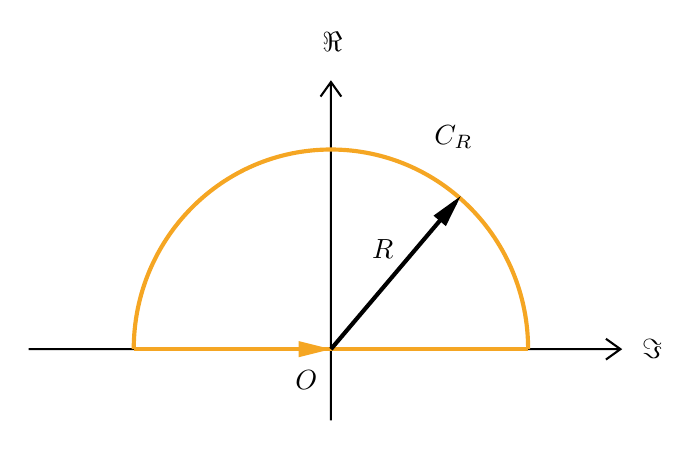
\begin{tikzpicture}[x=0.75pt,y=0.75pt,yscale=-1,xscale=1]
%uncomment if require: \path (0,266); %set diagram left start at 0, and has height of 266

%Shape: Axis 2D [id:dp1282392211894816] 
\draw  (162,181.79) -- (447.09,181.79)(307.61,53.09) -- (307.61,216.09) (440.09,176.79) -- (447.09,181.79) -- (440.09,186.79) (302.61,60.09) -- (307.61,53.09) -- (312.61,60.09)  ;
%Shape: Arc [id:dp1814309272431356] 
\draw  [draw opacity=0][line width=1.5]  (212.6,181.79) .. controls (212.6,181.79) and (212.6,181.79) .. (212.6,181.79) .. controls (212.6,128.66) and (255.14,85.6) .. (307.61,85.6) .. controls (360.08,85.6) and (402.61,128.66) .. (402.61,181.79) -- (307.61,181.79) -- cycle ; \draw  [color={rgb, 255:red, 245; green, 166; blue, 35 }  ,draw opacity=1 ][line width=1.5]  (212.6,181.79) .. controls (212.6,181.79) and (212.6,181.79) .. (212.6,181.79) .. controls (212.6,128.66) and (255.14,85.6) .. (307.61,85.6) .. controls (360.08,85.6) and (402.61,128.66) .. (402.61,181.79) ;  
%Straight Lines [id:da15038694853465828] 
\draw [color={rgb, 255:red, 245; green, 166; blue, 35 }  ,draw opacity=1 ][line width=1.5]    (212.6,181.79) -- (402.61,181.79) ;
\draw [shift={(307.61,181.79)}, rotate = 180] [fill={rgb, 255:red, 245; green, 166; blue, 35 }  ,fill opacity=1 ][line width=0.08]  [draw opacity=0] (15.6,-3.9) -- (0,0) -- (15.6,3.9) -- cycle    ;
%Straight Lines [id:da12449754393780421] 
\draw [color={rgb, 255:red, 0; green, 0; blue, 0 }  ,draw opacity=1 ][line width=1.5]    (307.61,181.79) -- (352.62,128.69) -- (367.5,111.14) ;
\draw [shift={(370.09,108.09)}, rotate = 130.29] [fill={rgb, 255:red, 0; green, 0; blue, 0 }  ,fill opacity=1 ][line width=0.08]  [draw opacity=0] (15.6,-3.9) -- (0,0) -- (15.6,3.9) -- cycle    ;


% Text Node
\draw (289,190.4) node [anchor=north west][inner sep=0.75pt]    {$O$};
% Text Node
\draw (302,27.4) node [anchor=north west][inner sep=0.75pt]    {$\Re $};
% Text Node
\draw (456,175.4) node [anchor=north west][inner sep=0.75pt]    {$\Im $};
% Text Node
\draw (326,127.4) node [anchor=north west][inner sep=0.75pt]    {$R$};
% Text Node
\draw (356,72.4) node [anchor=north west][inner sep=0.75pt]    {$C_{R}$};

% \draw   (239.6, 212.79) circle [x radius= 5, y radius= 5]  (234.6,212.79) -- (244.6,212.79)(239.6,207.79) -- (239.6,217.79) ;
% \draw   (334.61, 116.6) circle [x radius= 5, y radius= 5]  (329.61,116.6) -- (339.61,116.6)(334.61,111.6) -- (334.61,121.6) ;
% \draw   (429.61, 212.79) circle [x radius= 5, y radius= 5]  (424.61,212.79) -- (434.61,212.79)(429.61,207.79) -- (429.61,217.79) ;
% \draw   (396.48, 139.8) circle [x radius= 5, y radius= 5]  (391.48,139.8) -- (401.48,139.8)(396.48,134.8) -- (396.48,144.8) ;
\end{tikzpicture}


    \caption{半圆路径.}
    \label{fig:semicircle}
\end{figure}
下面证明上式第二项为零.一般的对于任意$\theta_1 \leq \theta \leq \theta_2$, 
有$\lim_{R\to \infty} zf(z) = 0$,可以证明对于该角度对应的圆弧$C$有,
\begin{equation}
    \lim_{R \rightarrow \infty} \int_C f(z) dz = 0 .
\end{equation}

\[
    \begin{aligned}
    \lim _{R \rightarrow \infty}\left|\int_C f(z) d z\right| \leq \int_{\theta_1}^{\theta_2} \lim _{R \rightarrow \infty}\left|f\left(R e^{i \theta}\right) i R e^{i \theta}\right| & d \theta \\
    & \leq\left(\theta_2-\theta_1\right) \lim _{R \rightarrow \infty}\left|f\left(R e^{i \theta}\right) R e^{i \theta}\right|=0 .
    \end{aligned}
\]
也就是说,
\begin{equation}
    \int_{-R}^R f(x) d x = 2\pi \imath  \sum_{z_j\in \textrm{上半平面}} \Res f(z_j),
\end{equation}

\begin{example}
    计算\[ 
    I = \int_{-\infty}^{\infty} \frac{dx}{1 + x^2}   .
    \]
\end{example}
\begin{solution}
    由$f(z) = \frac{1}{1+ x^2} = \frac{1}{(z-\imath)(z+\imath)}$可知
    其单极点$\pm \imath$,其中$\imath$在上半平面.
    \[
      \Res f(+\imath) = \frac{1}{2\imath}  
    \]
    因此,$I = 2\pi \imath  \frac{1}{2\imath} = \pi$.由于该积分是一个常见积分
    亦可以通过原函数$\arctan(x)$得到.留数定理的还可以计算这样的积分,
    \[
      I\int_{-\infty}^{\infty} \frac{dx}{(1 + x^2)^n} 
    \]
    具体求解过程参考梁昆淼数学物理方法的解.
\end{solution}


 \subsection{带复指数的定积分}
 考虑以下类型的定积分
 \begin{equation}
    I=\int_{-\infty}^{\infty} f(x) e^{\imath m x} d x
\end{equation}
其中,$m$为正实数;$f(z)$在上半平面除有限个奇点外是解析的,且$\lim_{|z|\to \infty} f(z) = 0, 0 \leq arg z \leq \pi$.
我们使用同样的半圆路径,类似的可以通过留数定理将实轴的积分转换为环路积分求得.
为了使用留数定理,我们先需要证明在半圆上的路径积分为零,这里就要用到\textbf{约旦引理}(Jordan lemma
).
即证明
\begin{equation}
    \lim _{R \rightarrow \infty} \int_{C_R} f(z) e^{\imath m z} d z=0 .
\end{equation}
当$R$足够大时,我们有$|f(z)| < \epsilon$.半圆积分
\begin{align}
    I_R&=\int_0^\pi f\left(R e^{\imath \theta}\right) 
    e^{\imath m R \cos \theta- m R \sin \theta} \imath R e^{\imath \theta} d \theta
    \\
    &\leq \epsilon R \int_0^\pi e^{-m R \sin \theta} d \theta=2 \epsilon R \int_0^{\pi / 2} e^{-m R \sin \theta} d \theta,
\end{align}
可以发现在$\left[ 0, \pi/2\right]$时,
\begin{equation}
    \frac{2}{\pi}\theta \leq \sin{\theta},
\end{equation}
于是有
\begin{equation}
    I_R \leq 2 \epsilon R \int_0^{\pi / 2} e^{-2 m R \theta / \pi} d \theta=2 \epsilon R \frac{1-e^{-m R}}{2 m R / \pi}<\frac{\pi}{m} \epsilon
\end{equation}
即
\begin{equation}
    \lim_{R\to \infty} I_R = 0.
\end{equation}
回到定积分$I$,可以得
\begin{equation}
    \label{eq:complex_exponential_integral}
    I=\int_{-\infty}^{\infty} f(x) e^{ \imath m x} d x = 2\pi \imath \sum_{z_j \in \text{上半平面}} \Res e^{\imath m z_j} f(z_j)
\end{equation}

对于以下类型的积分,可以利用上述结论.如
\begin{equation}
    \int_{0}^{\infty} f(x) \cos {m x} dx, \int_{0}^{\infty} G(x) \sin{m x} dx
\end{equation}
其中,$F(z)$为偶函数,$G(z)$为奇函数,它们在实轴上没有奇点,上半平面上除有限个奇点外解析.
很容易通过$\cos{mx} = \frac{1}{2}\left( e^{\imath m x} + e^{-\imath mx}\right)$等变换得到,即
$$
\begin{aligned}
\int_0^{\infty} F(x) \cos m x d x & =\int_0^{\infty} F(x) \frac{1}{2}\left(e^{\imath m x}+e^{-\imath m x}\right) d x \\
& =\frac{1}{2} \int_0^{\infty} F(x) e^{\imath m x} d x+\frac{1}{2} \int_0^{\infty} F(x) e^{-\imath m x} d x 
\\
& = \frac{1}{2} \int_{-\infty}^{\infty} F(x) e^{\imath m x} d x. 
\end{aligned}
$$

\begin{example}
计算 $\int_0^{\infty} \frac{\cos m x}{x^2+a^2} d x$.
\end{example}
\begin{solution}
偶函数$F(z) e^{\imath m z}=\frac{1}{z^2+a^2} e^{\imath m z}$ 有两个单极点 $\pm a \imath$, 其中 $+a \imath$ 在上半平面. 而 $e^{\imath m z} /\left(z^2+a^2\right)$ 在单极点 $+a \imath$ 的留数为
    $$
    \lim _{z \rightarrow a \imath}\left[(z-a \imath) \frac{e^{\imath m z}}{z^2+a^2}\right]=\lim _{z \rightarrow a \imath}\left[\frac{e^{\imath m z}}{z+a \imath}\right]=\frac{e^{-m a}}{2 a \imath}
    $$
    应用\eqref{eq:complex_exponential_integral},
    $$
    \int_0^{\infty} \frac{\cos m x}{x^2+a^2} d x=\pi \imath \frac{e^{-m a}}{2 a \imath}=\frac{\pi}{2 a} e^{-m a}.
    $$
\end{solution}
\section{Feynman技巧}
我们将讨论下面几个计算定积分的技巧。

\subsection{复变量代换}
以一个例子说明复变量代换的方法。求解定积分
\[
    I =  \int_0^{\infty} e^{-a x} \cos b x d x \\
\]
利用$\cos{bx} = \frac{1}{2}\left( e^{\imath b x} + e^{-\imath bx}\right)$
\[    \begin{aligned}
    I= & \frac{1}{2} \int_{0}^{\infty} \left(e^{-(a-\imath b) x} + e^{-(a + \imath b) x} \right)  d x \\
    = & \frac{1}{2} \left( \frac{1}{a-\imath b} +  \frac{1}{a+\imath b} \right)\\
    = & \frac{a}{a^2+b^2}
\end{aligned}
\]

\subsection{参数微分}
求解定积分
\[
    I =  \int_0^{\infty} x e^{-a x} \cos b x d x \\
\]
我们令
\[
  S(a) =   \int_0^{\infty} e^{-a x} \cos b x d x 
\]
已知 $S(a) = \frac{a}{a^2+b^2}$,通过对$S(a)$对$a$的求导得到
\[
    I = - S'(a)  = \frac{a^2 - b^2}{(a^2 +b^2)^2}    
\]
对于一般的含参数的微分,我们有
\begin{equation}
    \begin{aligned}
    \frac{d}{d \alpha} \int_{x_1(\alpha)}^{x_2(\alpha)} f(x, \alpha) d x= & \int_{x_1}^{x_2} \frac{\partial}{\partial \alpha} f(x, \alpha) d x \\
    & \left[\frac{d x_2(\alpha)}{d \alpha} \right] f(x_2, \alpha)- 
    \left[\frac{d x_1(\alpha)}{d \alpha}\right] f(x_1, \alpha)
    \end{aligned}
\end{equation}

\subsection{被积函数添加函数因子}
求解定积分
\[
    I =  \int_0^{\infty} \frac{\sin{x}}{x} d x 
\]
可以通过乘以一个函数因子$e^{-a x}$来构造参数函数
\[
 S(a) =     \int_0^{\infty}  e^{-a x} \frac{\sin{x}}{x} d x 
\]
这样我们有
\[
  S'(a) = -  \int_0^{\infty}  e^{-a x} \sin{x} d x  = \frac{1}{1+a^2}
\]
对于$a \to \infty$, 有 $S(\infty) = 0$。
而$\frac{1}{1+x^2}$的原函数为$\arctan{x}$,因此
\[S(a) = - \arctan{a} + C\]
可确定$C = \frac{\pi}{2}$,因此我们有$S(a) = \frac{\pi}{2} - \arctan{\alpha}$。
因此,
\[
  I = S(0) = \frac{\pi}{2} \textrm{。}    
\]
该结果我们已通过留数定理求得。
\subsection{积分求解实例}

